\documentclass[12pt,initial,twoside,maitrise]{dms}
\usepackage[utf8]{inputenc} %Obligatoires
%\usepackage[T1]{fontenc}    %
\usepackage[dvipsnames]{xcolor}
\usepackage[scaled]{beramono}
\usepackage{ocr}
\usepackage[T1]{fontenc}
\usepackage{listings}
\usepackage{array}
\usepackage{algorithm2e}
\usepackage{amsmath}

% Footnotes
%\usepackage[symbol]{footmisc}
%\renewcommand{\thefootnote}{\fnsymbol{footnote}}

% Quotes
\usepackage{epigraph}
\beforeepigraphskip=-20pt
\afterepigraphskip=20pt
\renewcommand{\textflush}{flushepinormal}

% Trees
\usepackage{tikz}
\usepackage{tikz-qtree}

% Table Checks
\usepackage{booktabs}
\usepackage{pifont}
\usepackage{float}

\newcommand{\wmark}{\textcolor{orange}{\ding{45}}}
\newcommand{\cmark}{\textcolor{green!80!black}{\ding{51}}}
\newcommand{\xmark}{\textcolor{red}{\ding{55}}}

\newcommand{\mediumwell}[1]{\textcolor{green}{#1}}
\newcommand{\medium}[1]{\textcolor{yellow}{#1}}
\newcommand{\mediumrare}[1]{\textcolor{orange}{#1}}
\newcommand{\rare}[1]{\textcolor{red}{#1}}

% Table
\newcommand*\rot{\rotatebox{90}}

% Code listings
\lstdefinelanguage{Kotlin}{
    comment=[l]{//},
    commentstyle={\color{gray}\ttfamily},
    emph={delegate, filter, firstOrNull, forEach, it, lazy, map, mapNotNull, println, return@},
    emphstyle={\color{OrangeRed}},
    identifierstyle=\color{black},
    keywords={abstract, actual, as, as?, break, by, class, companion, continue, data, do, dynamic, else, enum, expect, false, final, for, fun, get, if, import, in, infix, interface, internal, is, null, object, open, operator, override, package, private, public, return, sealed, set, super, suspend, this, throw, true, try, typealias, val, var, vararg, when, where, while},
    keywordstyle={\color{NavyBlue}\bfseries},
    morecomment=[s]{/*}{*/},
    morestring=[b]",
    morestring=[s]{"""*}{*"""},
    ndkeywords={@Deprecated, @JvmField, @JvmName, @JvmOverloads, @JvmStatic, @JvmSynthetic, Array, Byte, Double, Float, Int, Integer, Iterable, Long, Runnable, Short, String},
    ndkeywordstyle={\color{BurntOrange}\bfseries},
    sensitive=true,
    stringstyle={\color{ForestGreen}\ttfamily},
}

\lstset{
    language=kotlin,
    basicstyle=\ttfamily\scriptsize,
    numberstyle=\footnotesize,
    numbers=left,
    backgroundcolor=\color{gray!10},
    frame=single,
    tabsize=2,
    rulecolor=\color{black!30},
    %title=\lstname,
    %escapeinside={\%*}{*)},
    breaklines=true,
    %breakatwhitespace=true,
    framextopmargin=2pt,
    framexbottommargin=2pt,
    %extendedchars=false,
    %keepspaces=true,
    %moredelim=**[is]{@}{@},
    inputencoding=utf8
}

\def\inline{\lstinline[basicstyle=\ttfamily]}

%% Packages utiles.
\usepackage{graphicx,amssymb,subfigure,icomma}
%% icomma       permet d'écrire les nombres décimaux en
%%                  français (p.ex. 1,23 plutôt que 1.23)
%% subfigure    simplifie l'inclusion de figures côtes-à-côtes

%% Packages parfois utiles.
%%\usepackage{dsfont,mathrsfs,color,url,verbatim,booktabs}
%% dsfont       symboles mathématiques \mathds
%% mathrsfs     plus de symboles mathématiques \mathscr
%% color        pour utiliser des couleurs (comparer avec <xcolor>)
%% url          permet l'écriture d'url
%% verbatim     pour écrire du code ou du texte tel quel
%% booktabs     plus de macros pour faire les tableaux
%%                  (voir documentation du package)

%% pour que la largeur de la légende des figures soit = \textwidth
\usepackage[labelfont=bf, width=\linewidth]{caption}

%% les 3 lignes suivante servent à l'affichage de l'index
%% dans le visionneur de pdf. <hyperref> et <bookmark>
%% devraient être les dernier package a être chargé,
%% donc chargez vos packages avant.
\usepackage{hyperref}  % Ajoute les hyperlien
\hypersetup{colorlinks=true,allcolors=black}
\usepackage{hypcap}
\usepackage{bookmark}

\newtheorem{cor}{\corollaryname}[section]
\newtheorem{deff}[cor]{\definitionname}
\newtheorem{ex}[cor]{\examplename}
\newtheorem{lem}[cor]{\lemmaname}
\newtheorem{prop}[cor]{Proposition}
\newtheorem{rem}[cor]{\remarkname}
\newtheorem{theo}[cor]{\theoremname}

\numberwithin{equation}{section}
\numberwithin{table}{chapter}
\numberwithin{figure}{chapter}

\renewcommand{\baselinestretch}{1.5}

\begin{document}

\version{1}


\title{Programming tools for intelligent systems\\
\small{with a case study in autonomous robotics}}

\author{Breandan Considine}

\copyrightyear{2019}

\department{D\'epartement d'informatique et de recherche op\'erationnelle}

\president{Nom du pr\'esident du jury}

\directeur{Nom du directeur de recherche}

%%\codirecteur{Nom du co-directeur}         % s'il y a lieu

\membrejury{Nom du membre de jury}

%%\examinateur{Nom de l'examinateur externe}   %obligatoire pour la these

%% \membresjury{Deuxième membre du jury}  % s'il y a lieu

%%  \plusmembresjury{Troisième membre du jury}    % s'il y a lieu

%%\repdoyen{Nom du représentant du doyen} %obligatoire pour la these

\dateacceptation{La date d'acceptation}

%%
%% Voici les disciplines possibles (voir avec votre directeur):
%% \sujet{statistique},
%% \sujet{mathématiques}, \orientation{mathématiques appliquées},
%% \orientation{mathématiques fondamentales}
%% \orientation{mathématiques de l'ingénieur} et
%% \orientation{mathématiques appliquées}

\sujet{Discipline}
%%\orientation{orientation}%Ce champ est optionnel

%%
%% Fin des variables à définir. La commande \maketitle créera votre
%% page titre.

\pagenumbering{roman}
\maketitle

% Pour générer la deuxième page titre, il faut appeler à nouveau \maketitle
% Cette page est optionnelle et son inclusion est laissé à la discrétion
% de l'étudiant et du directeur de recherche, ou de tout autre instance
% d'autorité.
%%\maketitle

%%------------------------------------------------- %
%%              pages iv                            %
%%------------------------------------------------- %

\chapter*{Summary}

%%------------------------------------------------- %
%%        page v --- Table de matieres              %
%%------------------------------------------------- %

% Pour un mémoire en anglais, changer pour
% \anglais. Noter qu'il faut une permission
% pour écrire son mémoire en anglais.
\anglais
% \cleardoublepage termine la page actuel et force TeX
% a poussé les éléments flottant (fig., tables, etc.) sur
% la page (normalement TeX les garde en suspend jusqu'à ce
% qu'il trouve un endroit approprié). Avec l'option <twoside>,
% la commande s'assure que la prochaine page de texte est sur
% le recto, pour l'impression. On l'utilise ici
% pour que TeX sache que la table des matières etc. soit
% sur la page qui suit.
%% TABLE DES MATIÈRES
\cleardoublepage
\pdfbookmark[chapter]{\contentsname}{toc}  % Crée un bouton sur
% la bar de navigation
\tableofcontents
% LISTE DES TABLES
\cleardoublepage
\phantomsection  % Crée une section invisible (utile pour les hyperliens)
\listoftables
% LISTE DES FIGURES
\cleardoublepage
\phantomsection
\listoffigures

\NoChapterPageNumber
\cleardoublepage
\pagenumbering{arabic}

\mediumwell{\chapter{Introduction}\label{ch:introduction}}

\setlength{\epigraphwidth}{0.9\textwidth}
\epigraph{Intelligent system: \textit{A computer system that uses techniques derived from artificial intelligence, particularly one in which such techniques are central to the operation of the system.}}{\begin{flushright}--Wikipedia\end{flushright}}

Computational complexity is of such concern in computer science that a great deal of the field is dedicated to understanding it through the lens of function analysis and information theory. In software engineering, researchers are primarily interested in the complexity of building software - the digital manifestation of algorithms on physical hardware. One type of software complexity is the cognitive effort required to understand a program’s source code, which can be approximated by metrics such as cyclomatic or Halstead complexity.  While today’s software is more intelligent than ever before, it shows few signs of becoming more intelligible, and better tools are needed for managing the inherent complexity in building software systems.

\textit{The objective of writing this thesis is to develop methods that reduce the cognitive effort required to build intelligent systems, using developer tools, programming language abstractions, automated testing, and container-based virtualization.}

Broadly speaking, intelligent systems differ from ordinary software systems in that they enable machines to detect patterns, perform tasks, and solve problems which they are not explicitly programmed to solve and which human experts were previously incapable of solving by hard-coding explicit rules. Typically, these systems are able to:

\begin{enumerate}
    \item learn generalizable rules by processing large amounts of data
    \item tune a large number of free parameters (thousands to billions)
    \item outperform well-trained humans in domain specific tasks
\end{enumerate}

While the idea of intelligent systems has been around for decades, three critical developments made modern intelligent systems ultimately successful. First, computer processing power has become faster, cheaper, and much more readily available. Similarly, the digitalization of new datasets has made vast amounts of information available, and data storage costs have plummeted dramatically. (A \$5 thumb drive today has 200 times more storage capacity than a 2,000 pound, 5 MB, IBM hard drive that leased for \$3,000/mo. in 1956.) Most importantly, has been the development of more efficient learning algorithms.

In recent years, computer science and software engineering has made significant strides in building and deploying intelligent systems. Nearly every mobile computer in the world is able to detect objects in images, perform speech-to-text and language translation. These breakthroughs were the direct result of fundamental progress in neural networks and representation learning. Also key to the success of modern intelligent systems was the adoption of collaborative open source practices, pioneered by the software engineering community. Software engineers developed automatic differentiation libraries like Theano~\cite{theano}, Torch~\cite{collobert2002torch} and Caffe~\cite{jia2014caffe}, and built many popular simulators for reinforcement learning, the ease of use and availability of which was crucial for popularizing these techniques.

In this thesis, we explore several tools that facilitate the process of programming intelligent systems, and which reduce the cognitive effort required to understand an intelligent program. First, we demonstrate an integrated development environment that assists users writing robotics software (Chapter~\ref{ch:hatchery}). Next, we show a type-safe domain specific language for differentiable programming, an emerging paradigm in deep learning (Chapter~\ref{ch:kotlingrad}). To test this application, we use a set of techniques borrowed from property-based testing~\cite{fink1997property} and adversarial learning~\cite{lowd2005adversarial} (Chapter~\ref{ch:difftest}). Docker containers~\cite{merkel2014docker} are used to automate the building, testing and deployment of reproducible robotics applications on heterogeneous hardware platforms (Chapter~\ref{ch:ducker}). Finally, as a proof of concept for these ideas, we build an intelligent system comprised of a mobile autonomous vehicle and an Android mobile application, using the tools developed (Chapter~\ref{ch:case-study}).

\section{Stages in the software development lifecycle}\label{sec:sldc-stages}

\begin{figure}
    \centering
    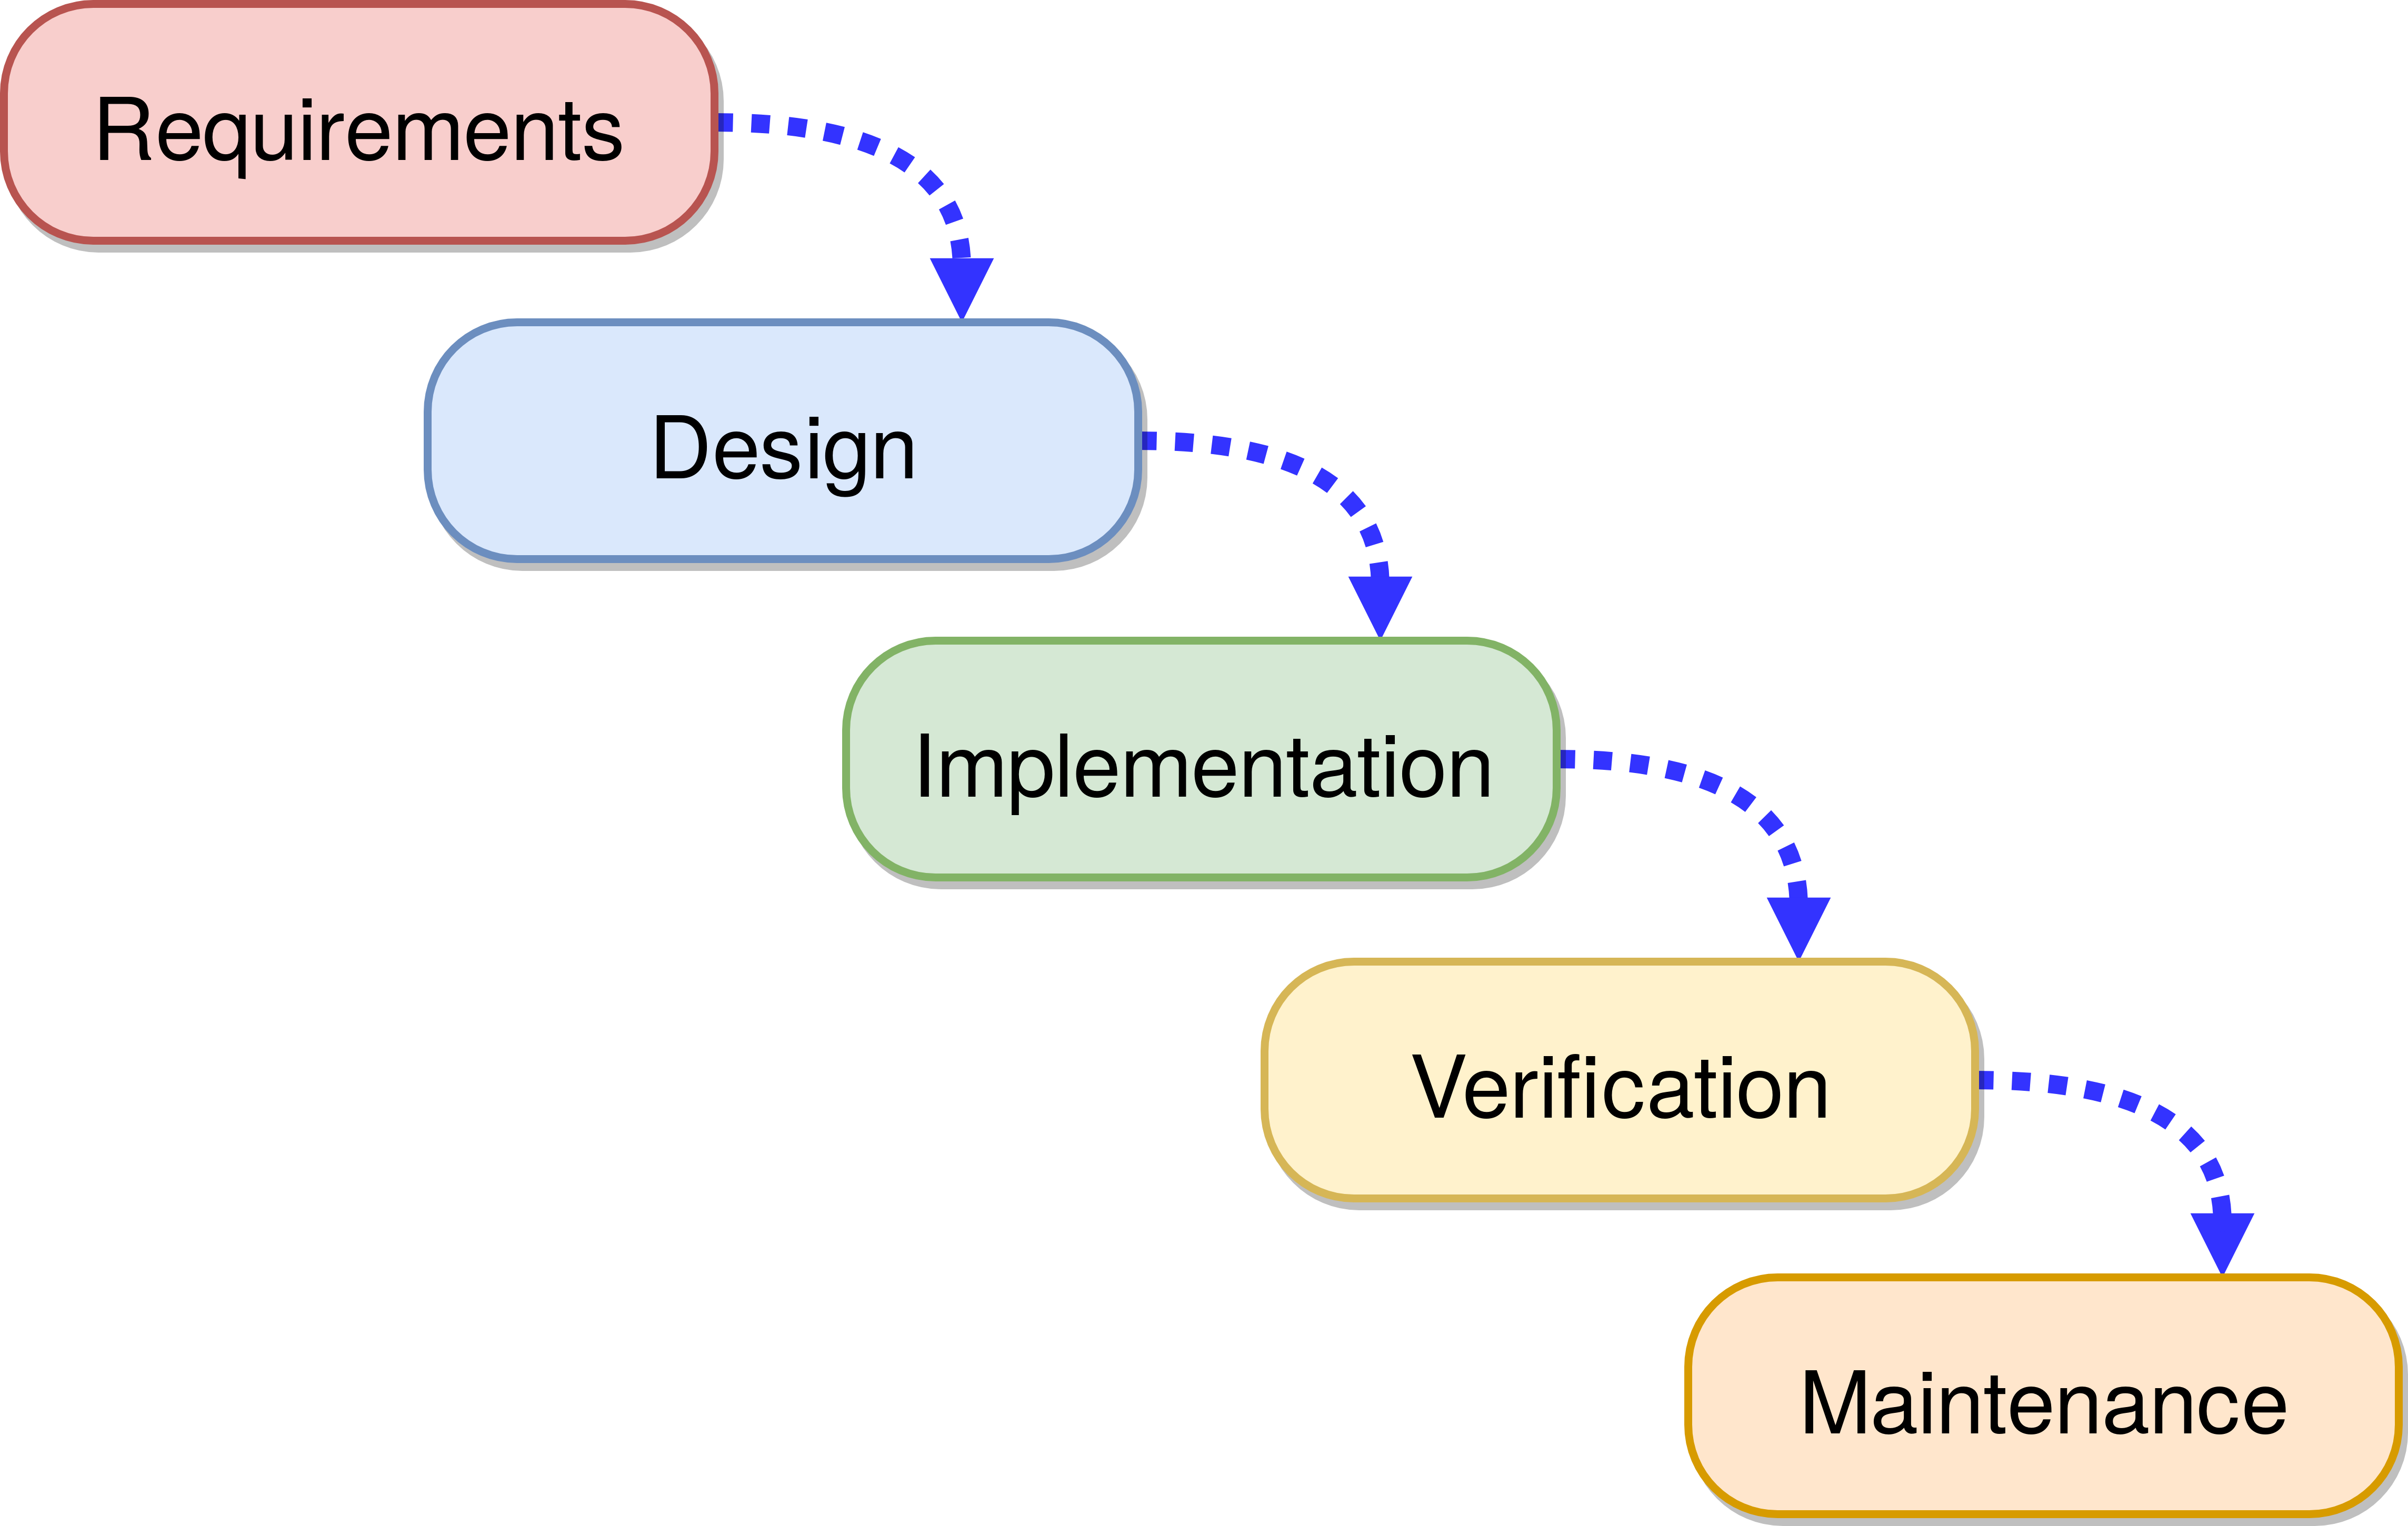
\includegraphics[width=0.70\textwidth]{waterfall_diagram.png}
    \caption{Royce's original Waterfall model, originally intended to describe the software development process, but the same sequence can be found in most engineering disciplines. We use it to help guide our discussion and frame our work inside of this process model.\vspace{-10}}
    \label{fig:waterfall_model}
\end{figure}

In traditional software engineering, the Waterfall Model~\ref{fig:waterfall_model} is a classical software process model comprised of five stages. While the Waterfall Model was an early model in software engineering, the same activities it describes can be found in most engineering process models. We propose contributions to four such areas: design in Chapter~\ref{ch:hatchery}, implementation in Chapter~\ref{ch:kotlingrad}, verification in Chapter~\ref{ch:difftest} and maintenance in Chapter~\ref{ch:ducker}.

\section{Designing intelligent systems}

Today's software systems are deeply complex entities. Gone are the days where a solitary programmer, even a very skilled one, can maintain a large software system alone. To effectively scale software systems, programmers must pool their mental capacity to form a knowledge graph. Software projects which rely on a small set of maintainers tend to perish due to the so-called \textit{bus factor}~\cite{cosentino2015assessing} - large portions of the knowledge graph are locked inside someone's head. Successful software projects learn how to distribute this graph and form new connections to the outside world. The knowledge graph which accumulates around a large software project contains facts, but it also contains workflows for programming, debugging, and delivery - all well-traveled paths through the labyrinth of software development. Components of this graph can be committed to writing in the form of documentation, but documentation is time-consuming and grows stale over time. What is needed is a system that preserves the benefits of documentation without the burdens of maintenance.

The development of software systems has a second component, the social graph. The social graph of a successful software project contains product designers, managers and software engineers who work in concert to build software that is well-designed, cohesive, and highly performant. Sometimes this means revising the specification to accommodate engineering challenges, or rewriting source code to remove technical debt. Software design is a multi-objective optimization process and requires contributors with a broad set of skills and common set of goals. To produce software that approximates criteria of its stakeholders, developers are asked to provide rapid prototypes, and continuously integrate user feedback. Yet today's software systems are larger and more unwieldy than ever. So finding ways to work together more efficiently is critical to building and maintaining intelligent systems.

First, let us consider the mechanical process of writing software with a keyboard.

Integrated development environments (IDEs) can assist developers building complex software applications by automating certain repetitive programming tasks. For example, IDEs perform static analyses and inspections for catching bugs quickly. They provide completion, refactoring and source code navigation, and they automate the process of building, running and debugging programs. While these tasks may seem trivial, their automation promises increased developer productivity by delivering earlier feedback, detecting clerical errors, and allows developers to focus on fundamental design tasks. Rather than being forced to concentrate on the structure and organization of text, if developers are able to manipulate code at a semantic level, they will be much happier and more productive. Furthermore, automating frequent tasks in software development, these mechanical tools enables them to focus on the fundamentals of writing and understanding programs.

But what are IDEs really doing? They are guiding developers through the knowledge graph of a software project. Consider what a new developer must learn to get up to speed: in addition to learning the language, developers must learn to use libraries and frameworks (arguably languages in their own right). They must become familiar with command line tools for software development, from build tools to version control and continuous integration. They must become familiar with the software ecosystem, programming styles, conventions and development workflows. And they must learn how to collaborate on a distributed team of developers. By automating common tasks in an interactive programming environment and making the graph connectivity explicit through document markup~\cite{goldfarb1981generalized} and projectional editing~\cite{voelter2014towards}, a well-designed IDE is a tool for graph traversal. It should come as no surprise IDEs are really graph databases.

In some aspects, the development of intelligent systems is no different than classical software engineering. While the former requires more human intervention, the same principles and best-practices which guide software engineering are also applicable to intelligent systems. And the same activities, from analysis, design, implementation, verification and maintenance will continue to play an important role in building intelligent systems. But in other aspects, the generic programming tools we use for developing traditional software will require domain-specific adaptations for machine learning to become a truly first class citizen in the next generation of software systems, particularly in the case of physically embodied agents. Towards that end, we propose \href{https://github.com/duckietown/hatchery}{Hatchery}, an IDE for the Robot Operating System (ROS), a popular robotics middleware.

\section{Implementation: Languages and compilers}

In the early days of machine learning, it was widely believed the development of human-level intelligence simply required a sufficiently descriptive first-order logic. By accumulating a database of facts and their relations, researchers believed they could use symbolic reasoning to bypass learning altogether. This rule-based approach dominated a large portion of early research in artificial intelligence and considerable effort was poured into the creation of domain-specific ontologies. Despite the best efforts of roboticists, signal processing engineers and natural language researchers, \textit{expert systems} were unable to scale to real-world applications, causing a great disillusionment in A.I. research for a number of decades. While they did not appreciate the difficulty of learning and were largely unsuccessful, expert systems excelled in areas where current machine learning systems struggle such as reasoning and interpretability, and there is reason to believe these ideas were ahead of their time.

What did finally work, is the idea of connectionist learning. By nesting random function approximators, called \textit{artificial neural networks} (ANNs), and training the system using backpropagation~\cite{werbos1990backpropagation, rumelhart1988learning}, the resulting system is capable of learning a surprising amount of intelligent behavior. The idea of neural network can be traced back to the mid-20th century~\cite{ivakhnenko1965cybernetic, rosenblatt1958perceptron}, but was not fully-realized in silico until after the widespread availability of cheap computing and large datasets~\cite{lecun2015deep}. In theory, a single layer of nesting is able to approximate any continuous differentiable function~\cite{hornik1989multilayer}, but in practice learning requires composing many such approximators in a deeply nested fashion, hence the term, \textit{deep neural networks} (DNNs). The importance of depth was suspected for many years, but the original backpropagation algorithm had difficulty on DNNs due to the vanishing gradient problem~\cite{bengio1994learning}. Solving this problem required a number of adaptations and many years to fully debug. It was not until 2013 when deep learning was competitive with humans in a number of domains.

While it took fundamental research in deep learning to realize the connectionist blueprint, the success of modern deep learning can be at least partly attributed to software tools for calculating derivatives, which are essential for the backpropagation. Although it has not been established if or how derivatives might be calculated in biological circuits, derivatives are essential for ANN training. For many years, the symbolic form of these derivatives had to be calculated manually when prototyping a new neural network architecture, a time-consuming and error-prone process. There is a well-known algorithm in the scientific computing community, called \textit{automatic differentiation} (A.D.)~\cite{linnainmaa1970representation, griewank1989automatic}, which is able to calculate derivatives for arbitrary differentiable functions. But surprisingly, it was not until much later, after the development of \textit{Theano}~\cite{theano} when AD became widely adopted in the machine learning community. This library alone greatly accelerated the pace of deep learning research and spurred the development of others like TensorFlow~\cite{abadi2016tensorflow} and PyTorch~\cite{paszke2017automatic}.

Intelligent systems engineers must think carefully about languages and abstractions. If developers are required to implement backpropogation by hand, they will have little time to think about the high-level characteristics of these systems. Similarly, if programming abstractions are too specific, small variations will require costly reimplementation. This is no different from traditional software engineering - as engineers, we need to choose the right abstractions for the task at hand. Too low-level and the design is lost in the details, too abstract and the details are lost completely. With deep learning, the necessity of choosing good abstractions is even more important, as the connection of between source code and runtime behavior is already difficult to grasp, due to the nature of neural networks.

\section{Testing: Verification and validation}

Most naturally arising phenomena, particularly those related to vision, planning and locomotion are high dimensional creatures. Richard Bellman famously coined this problem as the "curse of dimensionality". Our physical universe is populated by problems which are simple to pose, but impossible to solve inside of it. Claude Shannon, a contemporary of Bellman, calculated the number of unique chess games to exceed $10^{120}$, more than the number of atoms in the universe by approximately 40 orders of magnitude~\cite{shannon1950xxii}. At the time, it was believed that such problems would be insurmountable without a fundamental change in algorithms or computing machinery. Indeed, while Bellman or Shannon did not live to see the day, it took only half a century of progress in computer science before solutions to problems with the same order of complexity, first approximated in the Cambrian explosion 541 million years ago, were solved to a competitive margin in modern computers.

While computer science has made enormous strides in solving the common cases, Bellman's curse of dimensionality still haunts the long tail of machine learning, particularly for distributions that are highly disperse. Because the dimensionality of many real world problems we would like to solve is intractably large, it is difficult to be certain about the behavior of a candidate solution in all regimes. According to some studies, a human driver averages 1.09 fatalities per hundred million miles~\cite{kalra2016driving}. A new software build for an autonomous vehicle would need to accumulate 8.8 billion miles of driving in order to approximate the fatality rate of a human driver to within 20\% with a 95\% confidence interval. Deploying such a scheme in the real world would be logistically, not to mention ethically problematic.

Realistically, intelligent systems need better ways to practice their skills and probe the effectiveness of a candidate solution within a limited computational budget, without harming humans in the process. The goal of this testing is to highlight errors, but ultimately to provide feedback to the system. In software engineering, the real system under test is the ecosystem of humans and machines which provide each other's means of subsistence. The success of this arrangement depends on an external testing mechanism to enforce a minimum bar of rigor, typically some form of hardware- or human-in-the-loop testing. If the testing mechanism is not somehow opposed to the system under test, an intelligent system can deceive itself, which is neither in the system's nor its users' best interests.

\section{Software reproducibility and maitenance}

One of the challenges of building intelligent systems and programming in general, is the problem of reproducibility. Software reproducibility has a number of challenging aspects, including hardware compatibility, operating systems, file systems, build systems, and runtime determinism. While writing programs and feeding them directly into a computer may have once been sufficient, the source code of modern program are usually far too removed from its mechanical implementation to be meaningfully executed in isolation. Today's handwritten programs are like schematics for a traffic light - built in a factory, and which require a city's-worth of infrastructure, cars, and traffic laws. Like traffic lights, source code does not exist in a vacuum - built by compilers, interpreted by virtual machines, executed inside an operating system, and which following a certain protocol - programs are essentially meaningless abstractions outside this context.

As necessary in any good schematic, much of the information required to build a program is divided into layers of abstraction. Most low-level instructions carried out by a computer during the execution of a program were not written nor intended to be read by the programmer and have long since been automated and forgotten. In a modern programming language like Java, C\# or Python, the total information required to run a simple program often numbers in the trillions of bits. A portion of that data pertains to the software for building and running programs, including the build system, software dependencies, and development tools. Part of the data pertains to the operating system, firmware, drivers, and embedded software. And for most programs, such as those found in a typical GitHub repository, a vanishingly small fraction correspond to the handwritten program itself.

Applied machine learning shares many of the same practical challenges as traditional software development, with source code, release and dependency management. The current process of training a deep learning model can be seen as particularly long compilation step, but it differs significantly in that the source code is a high-level language which does not directly describe the computation being performed, but is a kind of meta-meta-program. The first meta-program describes the connectivity of a large directed graph (i.e.~ a computation graph or probabilistic graphical model), parameterized by weights and biases. The tuning of those parameters is another meta-program, describing the sequence of operations required to approximate a program which we do not have access, save for some input-output examples. Emerging techniques in meta-learning and hyper-parameter optimization (e.g.~differentiable architecture search~\cite{liu2018darts}) add even further meta-programming layers to this stack, by searching over the space of directed graphs themselves.

Hardware manufacturers have developed a variety of custom silicon to train and run these programs rapidly. But unlike most programming, deep learning is a much simpler model of computation - so long as a computer can add and multiply, it has the ability to run a deep neural network. Yet due to the variety of hardware platforms which exist and the software churn associated with them, reproducing deep learning models can be painstakingly difficult on new hardware, even with the same source code and dependencies. Many graph formats, or \textit{intermediate representations} (IRs) in compiler parlance, promise hardware portability but if developers are not careful, their models may not converge during training, or produce different results on different hardware. Complicating the problem, IRs are produced by competing vendors, with competing chips and incompatible standards (e.g.~MLIR, ONNX, NNEF, OpenVINO, et al.). While some have tried to leverage existing compilers such as GHC~\cite{elliott2018simple} or LLVM~\cite{wei2017dlvm}, there are few signs of convergence.

At the end of the day, researchers need to reproduce the work of other researchers, but the mental effort of re-implementing their abstractions can be tedious and detrimental towards scientific progress. Since it is necessary to reuse programs written by other researchers, it would be convenient if there were tools for reproducibility and incremental development. Fortunately, this is the same problem software developers have been attempting to solve for many years, via the open source community. But source control management (SCM) alone is insufficient, since SCM tools are primarily intended for text. While text-based representations may be stable for a time, as dependencies are periodically updated and rebuilt, important details about the original development environment can be misplaced. To reproduce a program in its entirety, we need a snapshot of all digital information available to the computer at the time of its execution. Short of that, the minimal set of dependencies for running a program is essential.

In order to mitigate the effects of software variability and assist the development of intelligent systems on heterogeneous platforms, we use a developer tool called Docker, part of a loosely-affiliated set of tools for build automation and developer operations which we shall refer to as \textit{container infrastructure}. Docker allows developers to freeze a software system and its host environment, allowing developers (e.g.~using a different environment) to quickly reproduce software on another computer. Docker itself is a technical solution, but also encompasses a growing set of best-practices which are procedural in nature. While this does not address the incompatibility of vendor standards and hardware drivers, it makes these variables explicit, and reduces the associated difficulty of reproducing software artifacts.

There is a second component to software reproducibility of intelligent systems, at the boundary of software and hardware. While today's simulators have become increasingly realistic, most roboticists agree that simulation alone will never be enough to capture the full distribution of real world data. In this view, while simulation can be a useful tool for detecting errors, it cannot fully reproduce all the subtleties of the real world, and must never be used as a surrogate for training on real-world data. Others have suggested a middle road~\cite{bousmalis2018using}, where judicious use of simulator training, alongside domain adaption is a sufficiently rigorous setting for training intelligent systems. Regardless of which view prevails, our goal is to provide rapid feedback to developers, and make this process as reproducible as possible.

\subsection{Case Study}\label{subsec:case-study}

All great software has a secret recipe: software gets better when engineers use the product. In the best case, software engineers are the core users, ideally by choice, if not by necessity. When software engineers are using their own software on a regular basis - bumping into sharp corners and encountering edge cases firsthand - the product gets better. When there is an obviously missing feature, it gets implemented. When there is a bug, it gets fixed. It may not be easy to find engineers who are so invested, or to build software which is so useful, but there must be some overlap in order for good software to become great. Termed "dogfooding"~\cite{harrison2006eating}, this practice has been used for public relations, but is an effective mechanism of building for self-improving cybernetic systems. It is also an important principle for open source software and safety-critical systems.

Putting this principle into practice, as the authors and primary users of these tools, we validate their effectiveness by developing a robotics application within the IDE (Chapter~\ref{ch:hatchery}), containing Kotlin$\nabla$ code (Chapter~\ref{ch:kotlingrad}), and which is is built using the Docker stack (Chapter~\ref{ch:ducker}).

\rare{\chapter{Design: Programming tools for robotics}\label{ch:hatchery}}
\setlength{\epigraphwidth}{0.78\textwidth}
\epigraph{``The hope is that, in not too many years, human brains and computing machines will be coupled together very tightly, and that the resulting partnership will think as no human brain has ever thought and process data in a way not approached by the information-handling machines we know today.''}{\begin{flushright}--J. C. R. Licklider, \textit{Man-Computer Symbiosis}~\cite{licklider1960man}\end{flushright}}

In this chapter we will discuss the design and implementation of an integrated development environment (IDE) for building intelligent robotic software. Modern robots are increasingly characterized by systems which learn and improve over time. Most researchers would agree that modern robotic systems have not yet achieved competitive sensorimotor abilities and most intelligent systems are not physically embodied. However, it is our view that any closed-loop control system not explicitly programmed for a given task, but learns it from experience is an intelligent system, and any closed-loop system with physical motors is a robotic system. While researchers have developed very successful methods in each type, it is believed that the intersection of these will be tremendously fruitful.

Hatchery is a tool designed to assist programmers writing robotics applications with ROS middleware. At the time of its release, \href{https://github.com/duckietown/hatchery}{Hatchery} was the first ROS plugin for the IntelliJ Platform \footnote{A popular IDE for C/C++, Python and Android development}, and one year later, is also the most widely used with close to 10,000 downloads. While the idea is simple, its prior absence and subsequent adoption suggest there is unmet demand for such tools in the development of intelligent software systems, particularly in robotics.

\section{Software architecture for robotics application}

The Robot Operating System (ROS) is a popular middleware for robotics applications. At its core, ROS provides software infrastructure for distributed messaging, but also includes a set of community-developed libraries and graphical tools for building robotics applications. ROS is not an operating system (OS) in the traditional sense, but it does offer OS-like functionality such as shared memory and inter-process communication. Unlike pure message-oriented systems like DDS and ZMQ, in addition to the communication infrastructure, ROS provides specific APIs for building decentralized robotic systems, particularly those which are capable of mobility. This includes standard libraries for serializing and consuming geometric data, coordinate frames, maps, sensor messages, and imagery.

A ROS application consists of several components, including the source code, configuration files, build infrastructure, compiled artifacts and the deployment environment. To build a ROS application, several steps are necessary. First, one must install the ROS system, which is only official supported on Debian-based Linux distributions. Then, a workspace must be created. ROS nodes, implemented as event based "talkers" and "listeners".

The ROS middleware provides several language front-ends for polyglot programming. According to one community census in 2018, 55\% of ROS applications on GitHub are written in C/C++, followed by Python at around 25\%~\cite{Areserio54:online}. Source code for a typical ROS application will include a mixture of C/C++ and Python code, roughly corresponding to the language preferences in the robotics and machine learning communities. Hatchery supports most common language front-ends for ROS, including Java, Python, C/C++, and several others, through the IntelliJ Platform. By targeting an IDE platform with support for polyglot programming, we are able to focus on language-agnostic features for the ROS ecosystem, such as parsing and editing ROS-specific configuration files, build and run configuration and other common development tasks.

\section{Foundations of a modern IDE}

To build an IDE, a few prerequisites are necessary. First, is an IDE, which we shall refer to as IDE\textsubscript{0}, and its source code. Assume that IDE\textsubscript{0} exists. In order to build a new IDE, IDE\textsubscript{1}, first load the source code from IDE\textsubscript{0} into IDE\textsubscript{0}. Then, using IDE\textsubscript{0}, modify and compile the source code. Finally, run the compiled artifact, which becomes IDE\textsubscript{1}. Iterate as necessary.

While valid, this approach has some disadvantages. First, most IDEs are already quite large and cumbersome to download, install, compile, and run. Since most plugins are small by comparison, modern IDEs have adopted a modular design, which allows them to load certain packages (i.e.\ \textit{plugins}), as needed. So most developers can skip the first step, and load such a plugin, using IDE\textsubscript{0} directly. It is still convenient to have the platform source code for reference purposes, but in most cases this source code is read-only.

\subsection{The parser}

An IDE consists of a few important components. First is a parser. This is typically not an ordinary parser, because most of the time users are modifying a program, their code is invalid. Even when the source code is invalid, the parser needs guide the user towards a functioning program. So this parser needs to be able to recover from syntactical errors.

We can parse URDF, package and launch XML, and srv files.

\subsection{Refactoring}

Refactoring support is implemented.

\subsection{Running and debugging}

Assistance for running ROS applications.

\section{More ROS Tools}

Detecting and managing ROS installations.

\mediumwell{\chapter{Implementation: languages and compilers}\label{ch:kotlingrad}}

\setlength{\epigraphwidth}{\textwidth}
\epigraph{``The derivative, as this notion appears in the elementary differential calculus, is a familiar mathematical example of a function for which both [the domain and the range] consist of functions.
''}{\begin{flushright}--Alonzo Church, 1941, \textit{The Calculi of Lambda Conversion
~\cite{church1985calculi}}\end{flushright}}

In this chapter, we will discuss the theory and implementation of a type safe domain specific language for automatic differentiation (AD), which has a variety of applications in numerical optimization and machine learning. The key idea behind AD is fairly simple. A small set of primitive operations form the basis for all modern computers, and by composing these operations over the real numbers in an orderly fashion, one can compute any computable function. In machine learning, it is often the case we are given a computable function, in the form of a program\footnote{Not all programs are computable functions, but all computable functions are programs.}, that does not work properly. We would like an algorithm for determining how to change the input slightly, so as to produce a more suitable output.

In 1964, such an algorithm was first conceived by Robert Wengert~\cite{wengert1964simple}, whose method is known today as forward-mode AD. Not long after, a certain Richard Bellman reproduced Wengert's algorithm to numerically estimate the orbital dynamics of a two body system, and recognized its potential for, "the treatment of large systems of differential equations which might not otherwise be undertaken"~\cite{bellman1965wengert}. Around the same time, key details of the backpropogation algorithm first emerged~\cite{dreyfus1990artificial}. In 1970, Seppo Linnainmaa~\cite{linnainmaa1970representation}, conceived the idea of calculating derivatives over computation graphs. Linnaimaa's algorithm was particularly important for the development of neural networks, and is today known as reverse-mode AD. But it was not until 2010 when standard software tools~\cite{bergstra2010theano, torch} for AD became widely available in machine learning. It is here where our journey begins.

\section{Automatic differentiation}\label{sec:automatic-differentiation}

Given some input to a function, AD tells us how to change the input by a minimal amount, in order to maximally change the outputs. Suppose we are handed a function $p_n: \mathbb{R}\rightarrow\mathbb{R}$, composed of a series of nested functions:
%
\begin{equation}
    p_n(p_0)= p_{n-1} \circ p_{n-2} \circ ... \circ p_1 \circ p_0
\end{equation}
%
From the chain rule of calculus, we recall that:
%
\begin{equation}
    \frac{dp_n}{dp_0} = {\displaystyle \prod_{i=1}^{n} \frac{dp_{i}}{dp_{i-1}}}
\end{equation}
%
Likewise, for a scalar function $Q(q_0, q_1, \dots, q_n):  \mathbb{R}^n\rightarrow\mathbb{R}$, the gradient $\nabla Q$ tells us:
%
\begin{equation}
    \nabla Q = \left( \frac{\partial Q}{\partial q_1}, \dots, \frac{\partial Q}{\partial q_n}\right)
\end{equation}
%
Occasionally, we may wish to compute the second-order partials for $Q$, i.e.\ the Hessian, $\mathbf{H}$:
%
\begin{equation}
\mathbf{H} = \begin{bmatrix}{\dfrac {\partial ^{2}Q}{\partial x_{1}^{2}}}&{\dfrac {\partial ^{2}Q}{\partial x_{1}\,\partial x_{2}}}&\cdots &{\dfrac {\partial ^{2}Q}{\partial x_{1}\,\partial x_{n}}}\\[2.2ex]{\dfrac {\partial ^{2}Q}{\partial x_{2}\,\partial x_{1}}}&{\dfrac {\partial ^{2}Q}{\partial x_{2}^{2}}}&\cdots &{\dfrac {\partial ^{2}Q}{\partial x_{2}\,\partial x_{n}}}\\[2.2ex]\vdots &\vdots &\ddots &\vdots \\[2.2ex]{\dfrac {\partial ^{2}Q}{\partial x_{n}\,\partial x_{1}}}&{\dfrac {\partial ^{2}Q}{\partial x_{n}\,\partial x_{2}}}&\cdots &{\dfrac {\partial ^{2}Q}{\partial x_{n}^{2}}}\end{bmatrix}
\end{equation}
%
More generally, for a vector function $\mathbf{f}:  \mathbb{R}^n\rightarrow\mathbb{R}^m$, the Jacobian $\mathbf J$ is defined as:
%
\begin{equation}
\mathbf J = \begin{bmatrix}
                       \dfrac{\partial \mathbf{f}}{\partial x_1} & \cdots & \dfrac{\partial \mathbf{f}}{\partial x_n} \end{bmatrix}
= \begin{bmatrix}
      \dfrac{\partial f_1}{\partial x_1} & \cdots & \dfrac{\partial f_1}{\partial x_n}\\
      \vdots & \ddots & \vdots\\
      \dfrac{\partial f_m}{\partial x_1} & \cdots & \dfrac{\partial f_m}{\partial x_n} \end{bmatrix}
    = \begin{bmatrix}
          \nabla f_1 \\
          \vdots \\
          \nabla f_n \end{bmatrix}
\end{equation}
%
For completeness, but rarely used in practice, is the second-order partials for vector functions:
%
\begin{equation}
\mathbf{H} (\mathbf {f} )=[\mathbf {H} (f_{1}), \mathbf {H} (f_{2}), \dots, \mathbf {H} (f_{m})]
\end{equation}
%
We can use these tools to compute the direction to adjust the inputs of a computable function, in order to maximally change that function's output, i.e.\ the direction of steepest descent.

\noindent Sometimes a function has the property that given an input $a$, no matter $a$ is changed, the output stays the same. We say that such functions have zero gradient for that input.
%
\begin{equation}
    (\nabla F)(a) \approx \mathbf{0}
\end{equation}
%
The cost of calculating the Hessian, $\mathbf{H}$ is approximately quadratic~\cite{griewank1993some} with respect to the number of independent variables under differentiation. If $\mathbf{H}(a)$ is tractable to compute and invertible, we could use the second-partial derivative test to determine that:\\
%
\begin{enumerate}
    \item If all eigenvalues of $\mathbf{H}(a)$ are positive, $a$ is a local minimum
    \item If all eigenvalues of $\mathbf{H}(a)$ are negative, $a$ is a local maximum
    \item If $\mathbf{H}$ contains a mixture of positive and negative eigenvalues, $a$ is a \textit{saddle point}\\
\end{enumerate}
%
For some classes of computable functions, small changes to the input will produce a sudden large change in the output. We say that such functions are non-differentiable.
%
\begin{equation}
    ||\nabla F|| \approx \pm \infty
\end{equation}
%
It is an open question whether non-differentiable functions exist in the real world~\cite{buniy2005hilbert}. At the current physical (10nm) and temporal (10ns) scale of modern computing, there exist no such functions, but modern computers are not equipped with the capability to accurately report the true value of their binary-valued functions, so for all intents and purposes, programs implemented by most physical computers are discrete relations. Nevertheless, computers are capable of approximating bounded functions of $\bathbb{R}^n$ to arbitrary precision given enough time and space. For most applications, a fixed precision approximation is sufficient.

There exists at the heart of machine learning a theorem that states a simple family of functions, which compute a weighted sum of a non-linear function $\varphi: R \rightarrow R$ composed with a linear function $\theta^\intercal x + b$, can approximate any bounded function on $\mathbb{R}^m$ to arbitrary precision. More precisely, the universal approximation theorem~\cite{hornik1989multilayer} states that for all real-valued continuous functions $f: C(\mathbb{I}_m)$, where $\mathbb{I}_m = [0, 1]^m$, there exists a function $\hat{f}$, parameterized by constants $n \in \mathbb{N}, \beta \in \mathbb{R}^n, b \in \mathbb{R}^n, \epsilon \in \mathbb{R}^+$ and $\theta \in \mathbb{R}^{m \times n}$:
%
\begin{equation}
    \begin{split}
        \hat{f}(x) = \beta^\intercal \varphi \left(\theta^\intercal x\right + b) \\
        \forall x\in I_m, \ | \hat{f}( x ) - f ( x ) | < \varepsilon
    \end{split}
\end{equation}
%
This theorem does not put an upper bound on the constant $n$, or tell us how to find $\theta$, somewhat limiting its practical applicability. But for reasons not yet fully understood, empirical results suggest it is possible to obtain accurate approximations to many naturally-arising functions in a relatively short time by composing these linear and non-linear functions in an alternating fashion and iteratively updating $\theta$ in the direction suggested by $\nabla_{\theta} \mathcal{L}(\hat{f}(x;\theta), f(x))$. In this setting, we do not have access to $f$ directly, but receive samples $Y = [f(x^{(1)}), \dots, f(x^{(k)})]$, which we try to obtain in as large a quantity as possible and run the following procedure:
%
\begin{equation}\label{eq:grad_descent}
    \begin{split}
        \theta \leftarrow \theta - \alpha\nabla_\theta\mathcal{L}(\hat{f}(X;\theta), Y)
    \end{split}
\end{equation}
%
For most common $\mathcal{L}$, the complexity of this procedure is linear with $k$. As $k$ can be quite large in practice, a single iteration of this procedure can take prohibitively long. Since obtaining the exact gradient is not very important, we use a stochastic variant by sampling a \textit{minibatch} of rows $X', Y'$, from $X, Y$, which is slightly noisier, but runs considerably more quickly.

\section{Differentiable programming}\label{sec:differentiable-programming}

\begin{figure}
    \centering
    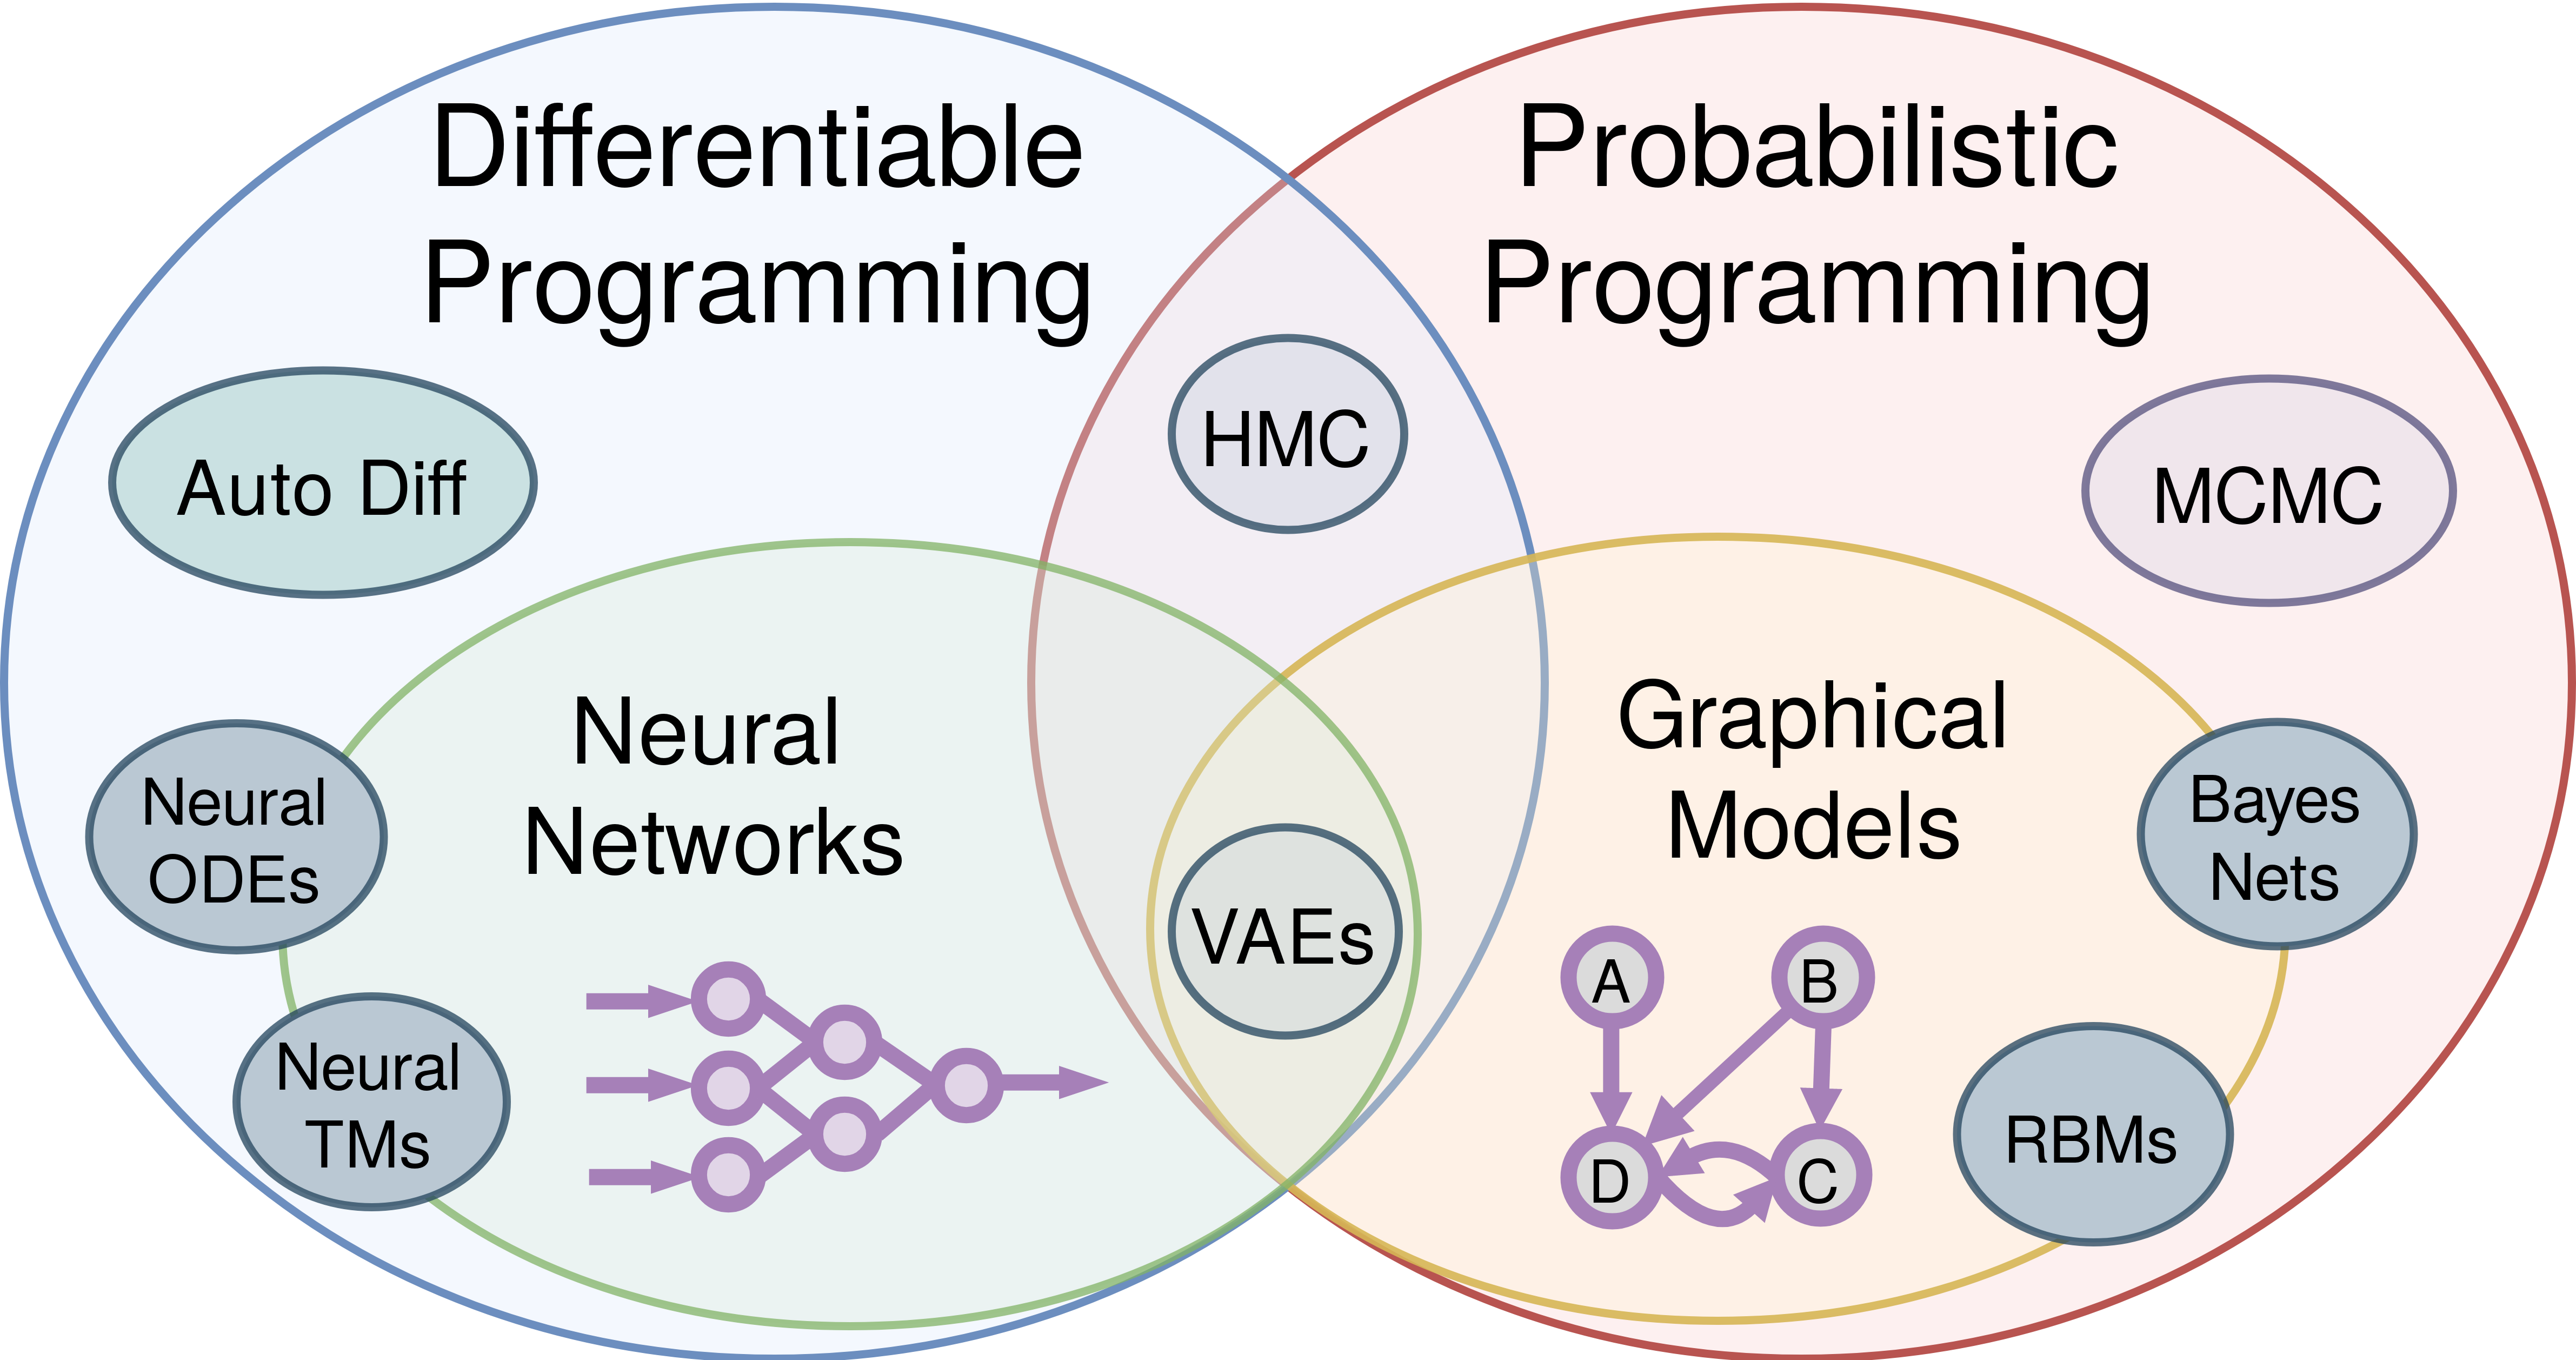
\includegraphics[width=0.90\textwidth]{diff_prob_prog.png}
    \caption{\textit{Differentiable programming} includes neural networks, but more broadly, arbitrary differentiable programs which use automatic differentiation and gradient-based optimization to approximate a loss function. \textit{Probabilistic programming} is a generalization of probabilistic graphical models, and uses various forms of Markov chain Monte Carlo (MCMC) and differentiable inference to approximate a probability density function.}
    \label{fig:diff_prob_prog}
\end{figure}

The renaissance of modern deep learning is widely attributed to progress in three research areas: algorithms, data and hardware. Among algorithms, most research has focused on deep learning architectures and representation learning. Equally important, arguably, is the role that automatic differentiation (AD) has played in facilitating the implementation of these ideas. Prior to the adoption of general-purpose AD libraries such as Theano, PyTorch and TensorFlow, gradients had to be derived manually. The widespread adoption of AD software simplified and accelerated the pace of gradient-based machine learning, allowing researchers to build deeper network architectures and new learning representations. Some of these ideas in turn, formed the basis for new methods in AD, which continues to be an active area of research in the programming language community.

A key aspect of the connectionist paradigm is learning neural representations via gradient descent. According to theory, for gradient descent to work, the representation must be differentiable almost everywhere. However many representations are non-differentiable in their natural domain. For example, the structure of language in its written form is not easily differentiable, as small changes to a word's symbolic representation can cause sudden changes to its semantic meaning. A key insight from deep learning is that many discrete data types can be mapped to a smoother latent space. For example, if we represent words as a vector of real numbers, then it is possible to define a mapping from the textual domain to their vector-based representation so that the semantic relations between words (as measured by their statistical co-occurrence in large language corpora) are geometrically preserved in vector space~\cite{pennington2014glove}. It so happens that many classes of discrete problems can be relaxed to continuous surrogates by using a good representation.

Around the same time, the deep learning community realized that perhaps strict differentiability was not so important all along. It was shown in practice, that computers using low-precision arithmetic such as 8-bit floating point ~\cite{wang2018training} and integer~\cite{jacob2018quantization} quantization are able to train neural networks without sacrificing performance. Strong assumptions like Lipschitz-continuity and $\beta$-smoothness once thought to be indispensable for gradient-based learning could be relaxed, as long as the noise introduced by quantization was negligible compared to stochastic gradient methods. In hindsight, this should not have come as a big surprise, since all digital computers use discrete representations anyway and were capable of training neural networks for nearly half a century. This suggests strict differentiability was not as important as having a good metric. As long as the loss surface permits metric learning, neural network training is surprisingly resilient to quantization.

As deep learning solved problems across various domains, researchers observed that neural networks were part of a broader class of differentiable architectures that could be designed, implemented and analyzed in a manner not unlike computer programs. Hence the term \textit{differentiable programming} (DP) was born. Today, DP has found a wide range of applications, from protein folding~\cite{alquraishi2018end}, to physics engines~\cite{de2018end,DBLP:journals_corr_DegraveHDW16} and graphics rendering~\cite{loper2014opendr} to meta-learning~\cite{liu2018darts}. These domains have well-studied dynamics models, with parameters that can be tuned via gradient descent. Traditionally, handcrafted optimization algorithms were required to learn these parameters, but given a smooth metric, DP promises to do this for a broad class of models, more or less automatically. For discrete optimization however, DP is not sufficient. To automatically learn discrete relations without ad hoc embedding, additional tools, such as probabilistic programming, are likely needed. As seen in Fig.~\ref{fig:diff_prob_prog}, these two fields have developed many productive collaborations in recent years.

\section{Static and dynamic languages}

Most programs in machine learning and scientific computing are written in dynamic languages, such as Python. In contrast, most of the industry uses statically typed languages~\cite{github}. Dynamically typed languages are popular for experimentation and prototyping. But are they scalable to building complex software systems? According to some studies, type related errors account for over 15\% of software bugs~\cite{gao2017type}. While the causality between statically typed languages and fewer bugs has not been conclusively established, the majority of robotics~\cite{Areserio54:online} and embedded systems today rely on statically typed languages.

Statically typed languages eliminate a broad class of runtime errors and allow us to reason about the behavior of programs without needing to run them. A well-designed library in a statically typed language will eliminate errors related to API misuse, which would otherwise require documentation and code samples. Finally, type systems make it easier to implement automated reasoning tools, which can provide more relevant autocompletion, source code navigation, and earlier detection of runtime errors.

\section{Imperative and functional languages}

Most programs written today are written in the imperative style, due the prevalence of the Turing Machine and von Neumann architecture~\cite{backus2007can}. $\lambda$-calculus provides an equivalent\footnote{In the sense that $\lambda$-calculus is Turing Complete.} language for computing, which we argue, is a more appropriate notation for expressing mathematical functions and computing their derivatives. In pure imperative programming the sole purpose of a function is to pass it values, and there is no way to refer to a function directly. More troubling in the case of automatic differentiation, is that imperative programs have mutable state, which requires taking extra precautions when computing mathematical derivatives.

In functional programming, the mathematical notion of function composition is a first-class pattern. Just like calculus, to take the derivative of a programming function composed with another function, we simply apply the chain rule~\ref{sec:automatic-differentiation}. Since there is no mutable state, we do not require any exotic data structures or compiler tricks to keep track of the program state.

For example, consider the vector function $f(l_1, l_2) = l_1 \cdot l_2$, seen in~\ref{tab:1}. Imperative programs, by allowing mutation, are destroying intermediate information. In order to recover the computation graph for reverse mode AD, we either need to override the assignment operator, or use a tape to store the intermediate values, which is quite tedious. In pure functional programming, mutable variables do not exist, which makes our lives much easier.

\begin{table*}[t]
    \centering
    \begin{tabular}{|l|l|}
        \hline
        Imperative & Functional \\
        \hline
        \begin{lstlisting}[language=Kotlin, linewidth=5.5cm]
fun dot(l1, l2) {
  if (len(l1) != len(l2))
    return error
  var sum = 0
  for(i in 0 to len(l1))
    sum += l1[i] * l2[i]
  return sum
}
        \end{lstlisting}
         &
        {\begin{lstlisting}[language=Kotlin, linewidth=5.5cm, numbers=none]
fun dot(l1, l2) {
  return if (len(l1) != len(l2))
    error
  else if (len(l1) == 0) 0
  else head(l1) * head(l2) +
    dot(tail(l1), tail(l2))
}
        \end{lstlisting}}
        \\
        \hline
    \end{tabular}
    \caption{Two programs, implementing the function $f(l_1, l_2) = l_1 \cdot l_2$.}
    \label{tab:1}
\end{table*}

Kotlin$\nabla$ treats mathematical functions and programming functions with the same underlying abstraction. Expressions are composed to form a data-flow graph (DFG). An expression is simply a \inline{Function}, which is only evaluated once invoked with numerical values, e.g. \inline{z(0, 0)}. In this way, Kotlin$\nabla$ is similar to other compiled graph based approaches like TensorFlow and Theano.

\section{Kotlin}\label{sec:kotlin}

When programming in a statically typed language, one common question is, "Given a value, \inline{x}, can \inline{x} be assigned to a variable of type \inline{Y}?" (e.g. \inline{x instanceof Y}) In Java, this question is both unsound~\cite{amin2016java} and undecidable~\cite{Grigore:2017:JGT:3009837.3009871} in the general case. It is possible to construct a Java program for which the answer is "yes" regardless of \inline{Y}, or which the answer cannot be determined in a finite amount of time.

Kotlin is a strong, statically typed language, that is well-suited for building cross-platform applications, with implementations in native, JVM, and JavaScript. Kotlin's type system~\cite{tate2013mixed} is strictly less expressive, but fully compatible with Java.

\section{Kotlin$\nabla$}\label{sec:kotlingrad}

Prior work has shown it is possible to encode a deterministic context-free grammar as a \textit{fluent interface}~\cite{gil2016formal} in Java. This result was strengthened to prove Java's type system is Turing complete~\cite{Grigore:2017:JGT:3009837.3009871}. As a practical consequence, we can use the same technique to perform shape-safe automatic differentiation (AD) in Java, using type-level programming. A similar technique is feasible in any language with generic types.

Differentiable programming has a rich history among dynamic languages like Python, Lua and JavaScript, with early implementations including projects like Theano~\cite{theano}, Torch~\cite{collobert2002torch}, and TensorFlow~\cite{abadi2016tensorflow}. Similar ideas have been implemented in statically typed, functional languages, such as Haskell's Stalin$\nabla$~\cite{pearlmutter2008using}, DiffSharp in F\#~\cite{baydin-diffsharp} and recently Swift~\cite{swift}. However, the majority of existing automatic differentiation (AD) libraries use a loosely-typed DSL, and few offer shape-safe tensor operations in a widely-used programming language.

Existing AD implementations for the JVM include Lantern~\cite{DBLP:journals-corr-abs-1803-10228}, Nexus~\cite{chen2017typesafe} and DeepLearning.scala~\cite{dl4s}, however these are Scala-based and do not interoperate with other JVM languages. Kotlin$\nabla$ is fully interoperable with vanilla Java, enabling broader adoption in neighboring languages. To our knowledge, Kotlin has no prior AD implementation. However, the language contains a number of desirable features for implementing a native AD framework. Kotlin$\nabla$ primarily relies on the following language features:

\begin{itemize}
\item \textbf{Operator overloading and infix functions} allow a concise notation for defining arithmetic operations on tensor-algebraic structures, i.e.\ groups, rings and fields.
\item \textbf{$\mathbf{\lambda}$-functions and coroutines} support functional differentiable programming with lambdas and shift-reset continuations, following~\cite{pearlmutter2008reverse} and~\cite{DBLP:journals-corr-abs-1803-10228}.
\item \textbf{Extension functions} support extending classes with new fields and methods and can be exposed to external callers without requiring sub-classing or inheritance.
\end{itemize}

\begin{figure}
    \centering
    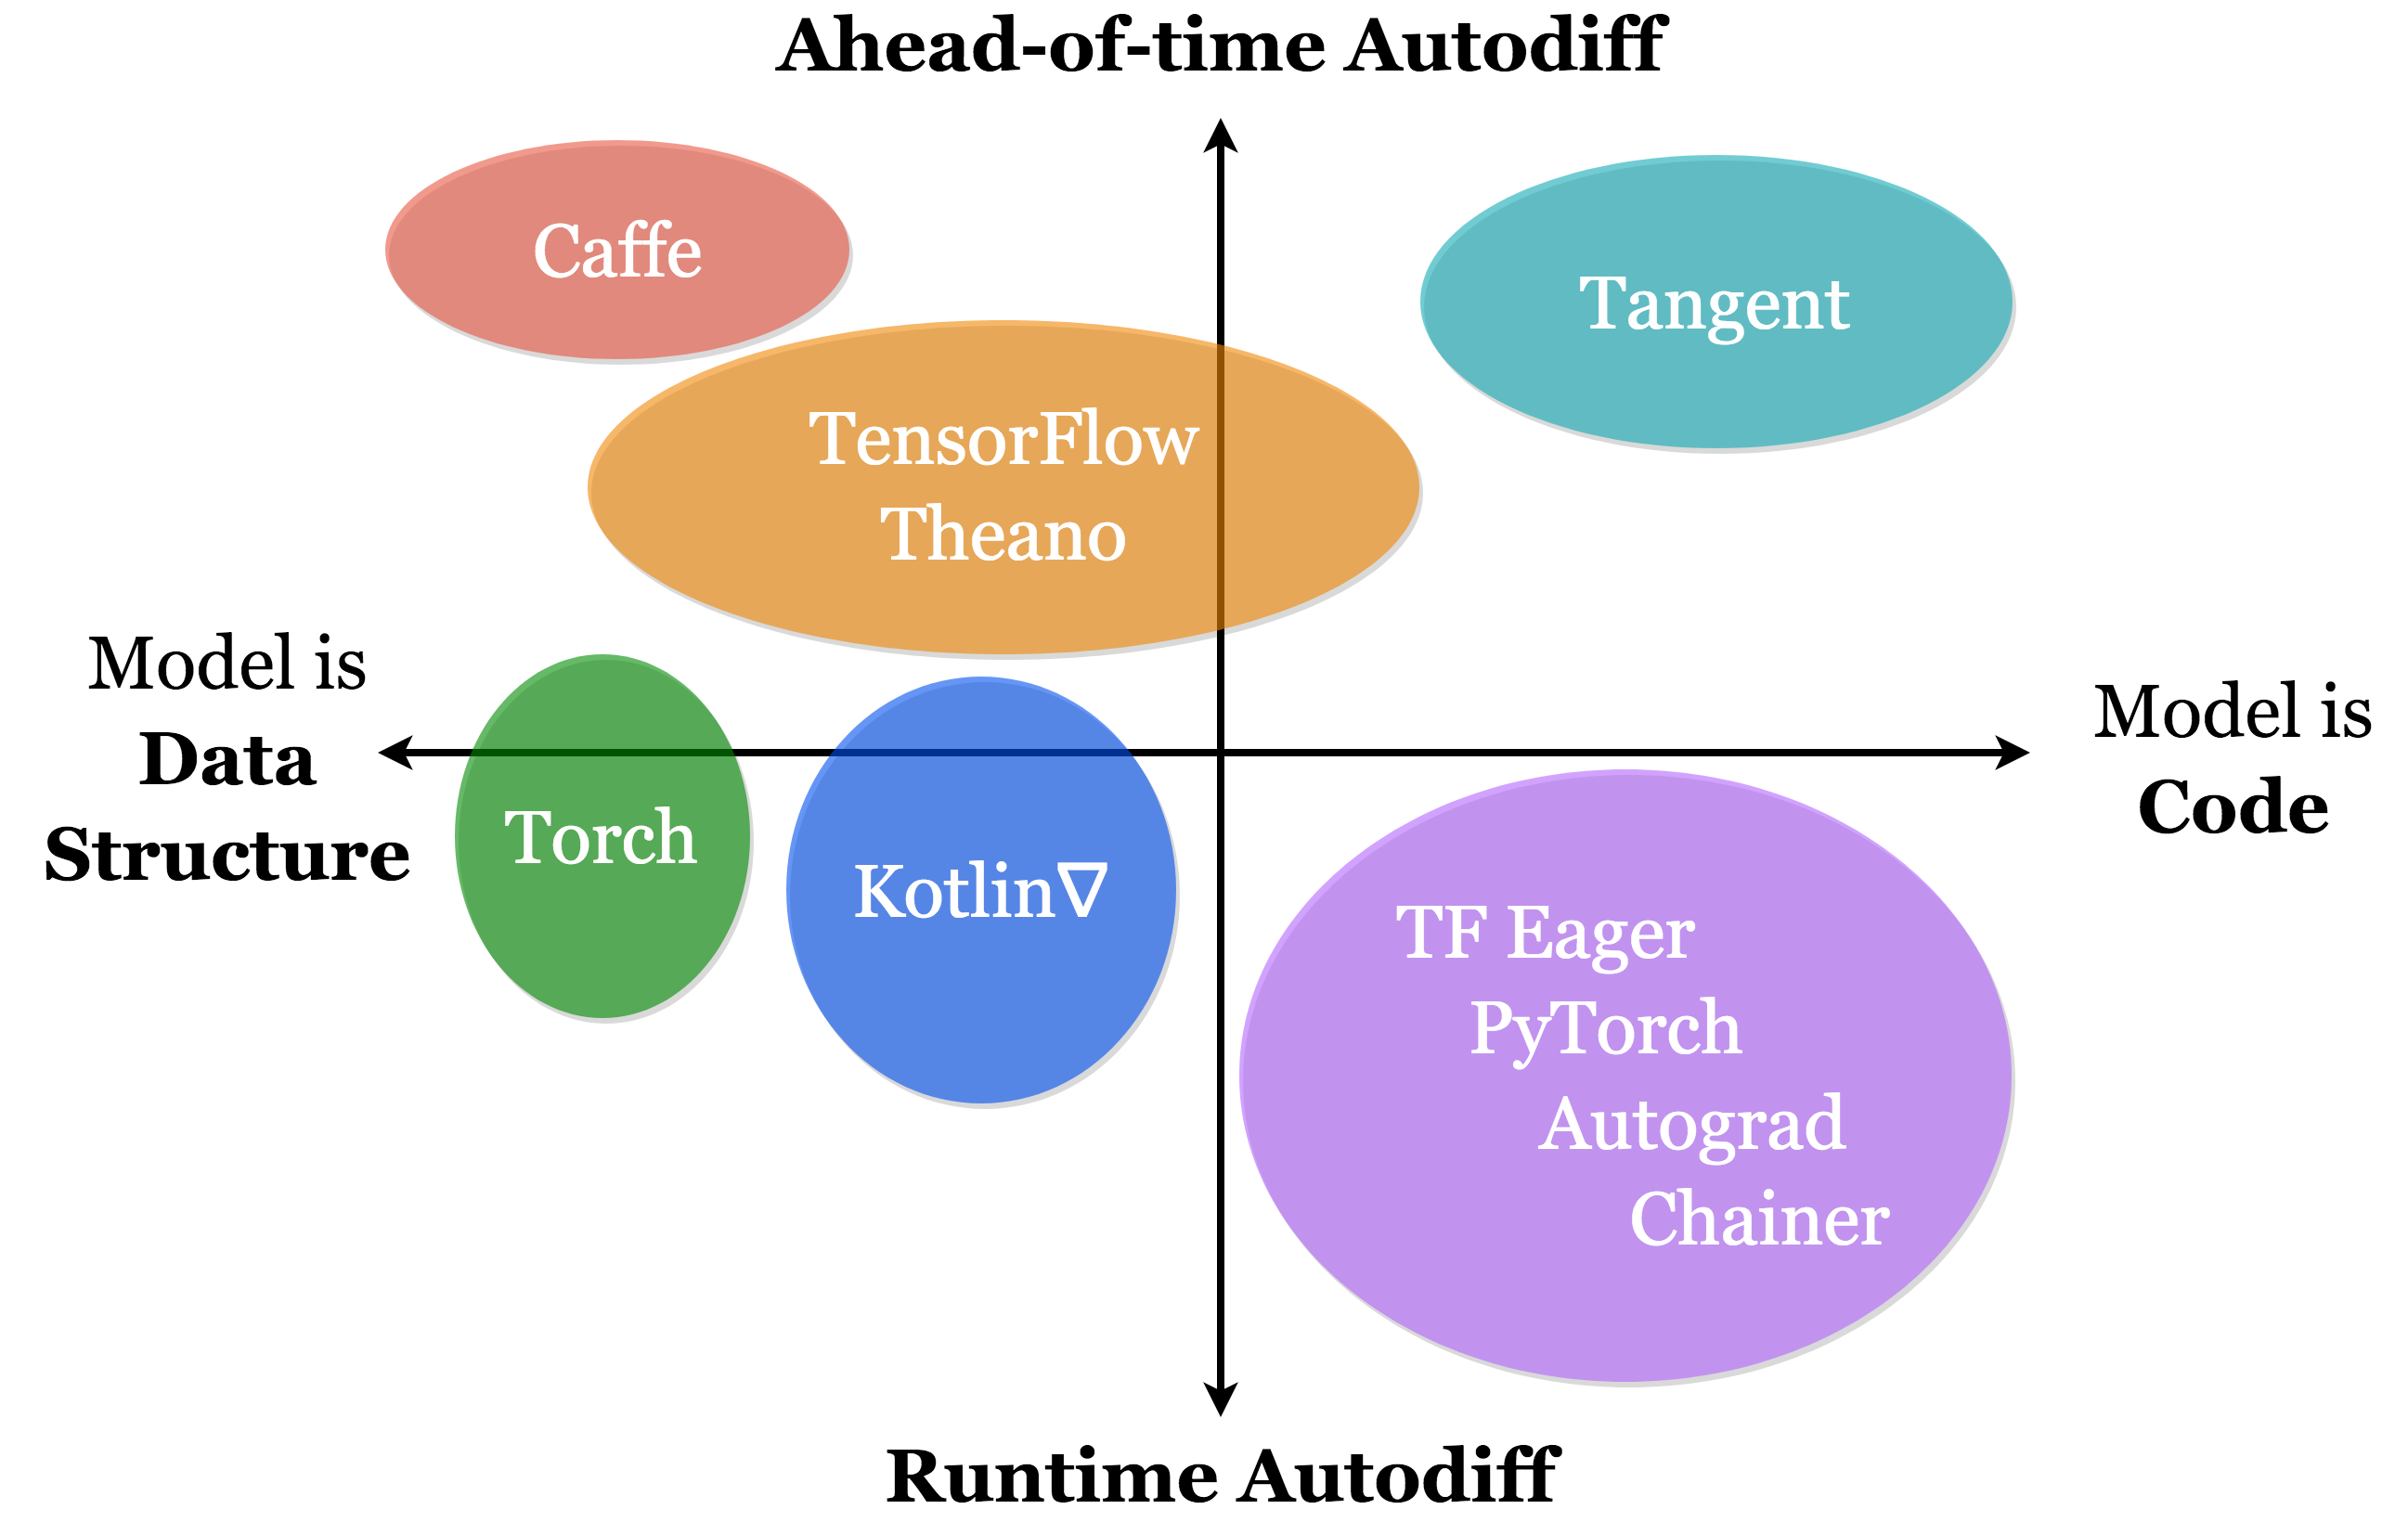
\includegraphics[width=0.70\textwidth]{kotlingrad_diagram.png}
    \caption{Adapted from~\cite{van2018tangent}. Kotlin$\nabla$ models are data structures, evaluated at runtime.}
    \label{fig:kotlingrad_digram}
\end{figure}

Kotlin$\nabla$ models are embedded domain specific languages (eDSLs), which are essentially data structures masquerading as code. These structures may look and act like code, but are really just functions building an abstract syntax tree (AST), which can be evaluated eagerly or lazily depending on the developer's needs. Typically these ASTs represent simple state machines, but they can also be used to implement a full-fledged programming language. Popular examples include SQL/LINQ~\cite{meijer2006linq}, OptiML~\cite{sujeeth2011optiml} and other fluent interfaces~\cite{fowler05fluent}. In a sufficiently expressive host language, one can implement any language as a library, without needing to write a lexer, parser, compiler or interpreter. And with a carefully designed type system, users will automatically receive code completion and static analysis from their favorite developer tools. Many have observed that functional programming languages are suitable host languages~\cite{elliott2003compiling,rompf2010lightweight}, perhaps owing to the notion of code as data \footnote{i.e.\ homoiconicity, notably introduced by Lisp, one of the first functional programming languages}.

\section{Usage}

Kotlin$\nabla$ allows users to implement differentiable programs by composing operations on numerical fields to form algebraic expressions. %Expressions are lazily evaluated inside a numerical context, which may be imported on a per file basis or lexically scoped for finer-grained control over the runtime behavior.
%
%
\begin{figure}[!htb]
\begin{lstlisting}[caption={A basic Kotlin$\nabla$ program with two inputs and one output, rendered below.},label={lst:basic_kotlingrad}, basicstyle=\ttfamily\small, language=Kotlin]
with(DoublePrecision) {   // Uses double precision numerics during evaluation
    val x = variable("x") // Declare immutable variables (these variables are
    val y = variable("y") // are just symbolic constructs for differentiation)
    val z = sin(10 * (x * x + pow(y, 2))) / 10 // Lazily evaluated expression
    val dz_dx = d(z) / d(x) // Support Leibniz's notation for differentiation
    val d2z_dxdy = d(dz_dx) / d(y) // Mixing higher order partial derivatives
    val d3z_d2xdy = grad(d2z_dxdy)[x] // Indexed gradient (same as d(f)/d(x))
    plot3D(d3z_d2xdy, -1.0, 1.0) // Plot result in 3-space (-1 < x, y, z < 1)
}
\end{lstlisting}
%    \centering $z = \sin{\big(10(x*x + y^2)\big)} / 10$, \texttt{plot}$\Big\left(\frac{\partial^{3z}}{\partial{x^2}\partial{y}}\Big\right)$ \\
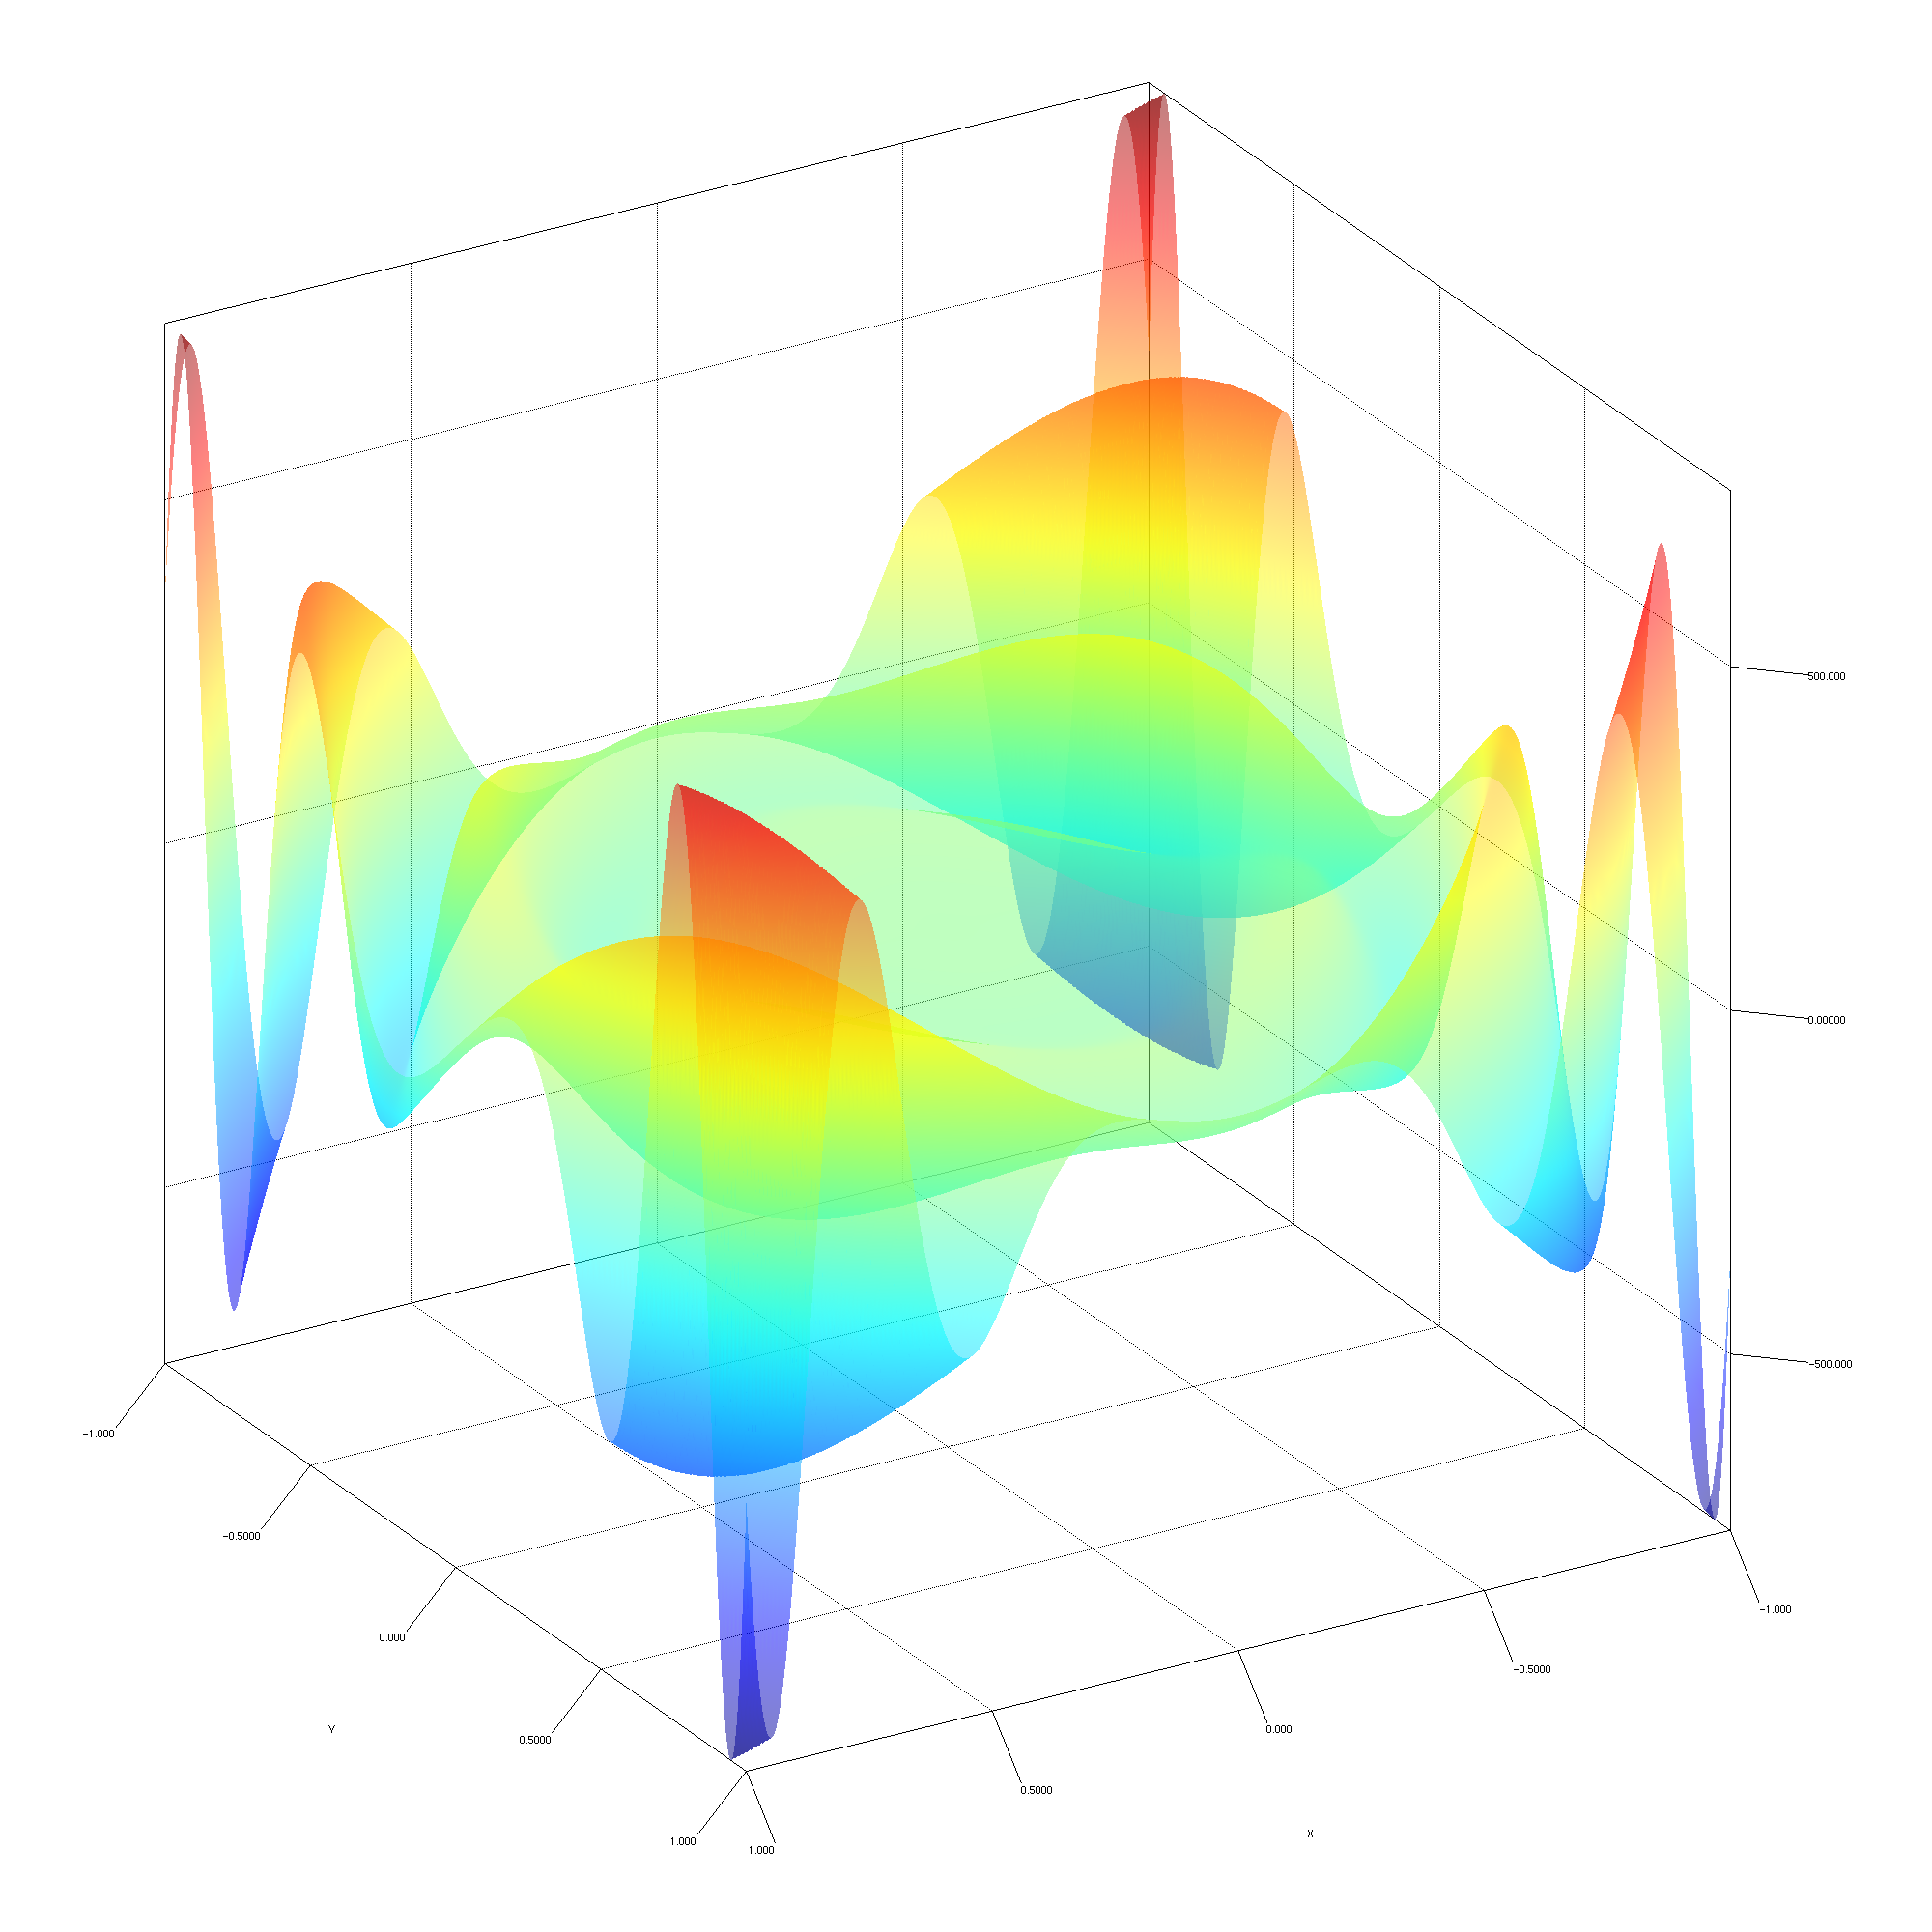
\includegraphics[scale=0.43]{plot_result.png}
\end{figure}
%
In Listing~\ref{lst:basic_kotlingrad}, we define a function with two variables and take a series of partial derivatives with respect to each variable. The function is numerically evaluated on the interval $(-1, 1)$ in each dimension and rendered in 3-space. % We can also plot higher dimensional manifolds (e.g.\ the loss surface of a neural network), projected into four dimensions, and rendered in three, where one axis is represented by time.
%
\begin{figure}[!htb]
\begin{lstlisting}[language=Kotlin, basicstyle=\ttfamily\footnotesize]
val z = sin(10 * (x * x + pow(y, 2))) / 10 // This does not perform any calculation
\end{lstlisting}
\centering
\begin{tikzpicture}[grow=left]
    \tikzset{level distance=45pt,sibling distance=-3pt}
    \Tree [.$\div$ [.\texttt{sin} [.$\times$ \texttt{10} [.$+$ [.$\times$ \texttt{\textbf{x}} \texttt{\textbf{x}} ] [.\texttt{pow} \texttt{\textbf{y}} \texttt{2} ] ] ] ] \texttt{10} ]
\end{tikzpicture}
\caption{Implicit DFG constructed by the original expression, \texttt{z} in Listing~\ref{lst:basic_kotlingrad}.}
    \label{lst:edsl}
\end{figure}

%It is possible to enforce shape-safe vector construction and checked vector arithmetic up to a fixed \texttt{L}. A similar pattern may be used to represent matrix and tensor data types, whose type signature will encode the operand's shape at runtime.

%In future work, we intend to implement a full grammar of differentiable primitives including matrix convolution, control flow and recursion. While Kotlin$\nabla$ currently implements arithmetic manually, we plan to wrap a BLAS such as cuBLAS or native linear algebra library for performance.

\section{Type system}\label{sec:type-system}

Early work in type safe dimension analysis can be found in Kennedy (1994~\cite{kennedy1994dimension}, 1996~\cite{kennedy1996programming}) showing how static types in array programming can be used to encode dimensionality and prevent common bugs arising from dimension mismatch. Kennedy's work is particularly interested in units of measurement, and was followed by Jay (1996~\cite{jay1996shape}), Rittri (1995~\cite{rittri1995dimension}), and Zenger (1997~\cite{zenger1997indexed}). Later, Kiselyov~\cite{kiselyov2005number,kiselyov2010fun} and Griffioen~\cite{griffioen2015type}, show how to encode numbers to infer array sizes in more complex ways. More recently, with the resurgence of interest in tensor algebra and the array programming paradigm, Chen (2017~\cite{chen2017typesafe}) and Rink (2018~\cite{rink2018modeling}) explore how shape safe tensor operations can be encoded in a sufficiently expressive type system.

The problem we would like to solve can be summarized as follows. Given two variables \texttt{x} and \texttt{y}, and operator $\diamond$, how do we determine whether the expression \texttt{z = x} $\diamond$ \texttt{y} is valid, and if so, what is the result type of \texttt{z}? For matrix multiplication, when $\texttt{x} \in \mathbb{R}^{m \times n}$ and $\texttt{y} \in \mathbb{R}^{n \times p}$, the expression is well-typed and we can infer $\texttt{z} \in \mathbb{R}^{m \times p}$. More generally, we would like to infer the type of \texttt{z} for some operator $\otimes: (\mathbb{R}^\mathbf{a}, \mathbb{R}^\mathbf{b}) \rightarrow \mathbb{R}^\mathbf{c}$ where $\mathbf{a} \in \mathbb{Z}^q, \mathbf{b} \in \mathbb{Z}^r, \mathbf{c} \in \mathbb{Z}^s$ and $q, r, s \in \mathbb{Z}^\geq$. For most linear algebra operations, $\mathcal{T}$ is computable in $\mathcal{O}(1)$ as in the case of standard matrix multiplication - we can simply check the inner dimensions for equivalence and use the outer dimensions for inference.

Shape checking matrix operations is not always decidable, however. For arbitrary type functions $\mathcal{T}(\mathbf{a}, \mathbf{b})$, checking $\mathcal{C}(\mathbf{a}, \mathbf{b}, \mathbf{c}) = \mathbf{c} \Leftrightarrow \mathcal{T}(\mathbf{a}, \mathbf{b})$ requires a Turing machine, at which point it would be easier to implement at runtime rather than in the type level. If $\mathcal{T}$ is allowed to use the multiplication operator, as in the case of convolutional arithmetic~\cite{dumoulin2016guide}, type checking becomes equivalent to Peano arithmetic, which is known to be undecidable~\cite{godel1931formal}.

First class dependent types are useful for ensuring arbitrary shape safety (e.g.\ when concatenating and reshaping matrices \cite{xi1998eliminating}), but they are unnecessary for simple equality checking (such as when multiplying two matrices)\footnote{Many less powerful type systems are still capable of performing arbitrary computation in the type checker. As specified, Java's type system is known to be Turing Complete~\cite{Grigore:2017:JGT:3009837.3009871}. It may be possible to emulate a limited form of dependent types in Java by exploiting this property, although this may not be computationally tractable due to the practical limitations noted by Grigore}. When the shape of a tensor is known at compile time, it is possible to type check arithmetical operations in a fully decidable type system, as long as the host language supports subtyping and parametric polymorphism. In practice, we can implement a shape-checked tensor arithmetic in Java, Kotlin, C++, C\# or Typescript.

{\tiny
\begin{table}
    \begin{tabular}{|c|c|c|c|l|}
        \hline
        \multicolumn{1}{|c|}{Math$\dagger$}                   &  Infix                                                                         &  Prefix                                                                                 & Postfix                                                                                    & Type                                                                                                                                                                                    \\ \hline
                 $A + B$                                      & \begin{tabular}{@{}c@{}}\texttt{a + b}\\\texttt{a.plus(b)}\end{tabular}        &  \texttt{plus(a, b)}                                                                    &                                                                                            & $ (\texttt{a}:  \mathbb{R}^{\tau}\rightarrow\mathbb{R}^{\pi}, \texttt{b}: \mathbb{R}^{\lambda} \rightarrow \mathbb{R}^{\pi}) \rightarrow (\mathbb{R}^{?}\rightarrow \mathbb{R}^{\pi}) $ \\ \hline
                 $A - B$                                      & \begin{tabular}{@{}c@{}}\texttt{a - b}\\\texttt{a.minus(b)}\end{tabular}       &  \texttt{minus(a, b)}                                                                   &                                                                                            & $ (\texttt{a}:  \mathbb{R}^{\tau}\rightarrow\mathbb{R}^{\pi}, \texttt{b}: \mathbb{R}^{\lambda} \rightarrow \mathbb{R}^{\pi}) \rightarrow (\mathbb{R}^{?}\rightarrow\mathbb{R}^{\pi})  $ \\ \hline
                 $A   B$                                      & \begin{tabular}{@{}c@{}}\texttt{a * b}\\\texttt{a.times(b)}\end{tabular}       &  \texttt{times(a, b)}                                                                   &                                                                                            & $ (\texttt{a}: \mathbb{R}^{\tau}\rightarrow\mathbb{R}^{m \times n}, \texttt{b}: \mathbb{R}^{\lambda}\rightarrow\mathbb{R}^{n \times p})    \rightarrow (\mathbb{R}^{?}\rightarrow\mathbb{R}^{m \times p})  $ \\ \hline
\begin{tabular}{@{}c@{}}$\frac{A}{B}$\\$AB^{-1}$\end{tabular} & \begin{tabular}{@{}c@{}}\texttt{a / b}\\\texttt{a.div(b)}\end{tabular}         &  \texttt{div(a, b)}                                                                     &                                                                                            & $ (\texttt{a}: \mathbb{R}^{\tau}\rightarrow\mathbb{R}^{m \times n}, \texttt{b}: \mathbb{R}^{\lambda}\rightarrow\mathbb{R}^{p \times n}) \rightarrow (\mathbb{R}^{?}\rightarrow\mathbb{R}^{m \times p})     $ \\ \hline
\begin{tabular}{@{}c@{}}$-A$\\$+A$\end{tabular}               &                                                                                &  \begin{tabular}{@{}c@{}}\texttt{-a}\\\texttt{+a}\end{tabular}                          & \begin{tabular}{@{}c@{}}\texttt{a.unaryMinus()}\\\texttt{a.unaryPlus()}\end{tabular}       & $                   (\texttt{a}: \mathbb{R}^{\tau}\rightarrow\mathbb{R}^{\pi}) \rightarrow (\mathbb{R}^{\tau}\rightarrow\mathbb{R}^{\pi})                                             $ \\ \hline
\begin{tabular}{@{}c@{}}A+1 \\ A-1\end{tabular}               & \begin{tabular}{@{}c@{}}\texttt{a + 1}\\\texttt{a - 1}\end{tabular}            &  \begin{tabular}{@{}c@{}}\texttt{++a}\\\texttt{--a}\end{tabular}                        & \begin{tabular}{@{}c@{}}\texttt{a++, a.inc()}\\\texttt{a--, a.dec()}\end{tabular}          & $                 (\texttt{a}: \mathbb{R}^{\tau}\rightarrow\mathbb{R}^{m \times m}) \rightarrow (\mathbb{R}^{\tau}\rightarrow\mathbb{R}^{m \times m})                                               $ \\ \hline
\begin{tabular}{@{}c@{}}sin(a)\\cos(a)\\tan(a)\end{tabular}   &                                                                                &  \begin{tabular}{@{}c@{}}\texttt{sin(a)}\\\texttt{cos(a)}\\\texttt{tan(a)}\end{tabular} & \begin{tabular}{@{}c@{}}\texttt{a.sin()}\\\texttt{a.cos()}\\\texttt{a.tan()}\end{tabular}  & $                                            (\texttt{a}: \mathbb{R}\rightarrow\mathbb{R}) \rightarrow (\mathbb{R}\rightarrow\mathbb{R})                                              $ \\ \hline
                $\ln(A)$                                      &                                                                                &  \begin{tabular}{@{}c@{}}\texttt{ln(a)}\\\texttt{log(a)}\end{tabular}                   & \begin{tabular}{@{}c@{}}\texttt{a.ln()}\\\texttt{a.log()}\end{tabular}                     & $                  (\texttt{a}: \mathbb{R}^{\tau}\rightarrow\mathbb{R}^{m \times m}) \rightarrow (\mathbb{R}^{\tau}\rightarrow\mathbb{R}^{m \times m})                                              $ \\ \hline
               $\log_b A$                                     & \texttt{a.log(b)}                                                              &  \texttt{log(a, b)}                                                                     &                                                                                            & $       (\texttt{a}: \mathbb{R}^{\tau}\rightarrow\mathbb{R}^{m \times m}, \texttt{b}: \mathbb{R}^{\lambda}\rightarrow\mathbb{R}^{m \times m}) \rightarrow (\mathbb{R}^{?}\rightarrow\mathbb{R})     $ \\ \hline
                $A^{b}$                                       & \texttt{a.pow(b)}                                                              &  \tettt{pow(a, b)}                                                                      &                                                                                            & $       (\texttt{a}: \mathbb{R}^{\tau}\rightarrow\mathbb{R}^{m \times m}, \texttt{b}: \mathbb{R}^{\lambda}\rightarrow\mathbb{R}) \rightarrow (\mathbb{R}^{?}\rightarrow\mathbb{R}^{m \times m})     $ \\ \hline
\begin{tabular}{@{}c@{}}$\sqrt{a}$\\$\sqrt[3]{a}$\end{tabular} & \begin{tabular}{@{}c@{}}\texttt{a.pow(1.0/2)}\\\texttt{a.root(3)}\end{tabular} &  \begin{tabular}{@{}c@{}}\texttt{a.pow(1.0/2)}\\\texttt{a.root(3)}\end{tabular}         & \begin{tabular}{@{}c@{}}\texttt{a.sqrt()}\\\texttt{a.cbrt()}\end{tabular}                  & $                        (\texttt{a}: \mathbb{R}^{\tau}\rightarrow\mathbb{R}^{m \times m}) \rightarrow (\mathbb{R}\rightarrow\mathbb{R}^{m \times m})                                               $ \\ \hline
\begin{tabular}{@{}c@{}}$\frac{da}{db}$\\$a'(b)$\end{tabular} & \texttt{a.diff(b)}                                                             &  \texttt{grad(a)[b]}                                                                    & \texttt{d(a) / d(b)}                                                                       & $                    (\texttt{a}: C(\mathbb{R}^{m})^{*}, \texttt{b}: \mathbb{R}\rightarrow\mathbb{R}) \rightarrow (\mathbb{R}^{m}\rightarrow\mathbb{R})                               $ \\ \hline
               $\nabla a$                                     &                                                                                &  \texttt{grad(a)}                                                                       & \texttt{a.grad()}                                                                          & $                   (\texttt{a}: C(\mathbb{R}^{m})) \rightarrow (\mathbb{R}^{m}\rightarrow\mathbb{R}^{m})                                                                         $ \\ \hline
    \end{tabular}
\end{table}
}
%$\dagger$ \texttt{a} and \texttt{b} are higher order functions. These may be constants (e.g. 0, 1.0), variables (e.g. \texttt{Var("x")}) or expressions (e.g. \texttt{x + 1}, \texttt{2 * x + y}).

\section{Shape safety}\label{sec:shape-safety}

\noindent There are three broad strategies for handling shape errors in array programming: \\
%
\begin{enumerate}
    \item Hide the error somehow by implicitly reshaping or broadcasting arrays
    \item Announce the error at runtime, with a relevant message, e.g.\ "InvalidArgument"
    \item Do not allow programs which can result in a shape error to compile \\
\end{enumerate}
%
In Kotlin$\nabla$, we use the third strategy. Consider the following program:
%
\begin{lstlisting}[language=Kotlin]
val a = Vec(1.0, 2.0) // Inferred type: Vec<Int, `2`>
val b = Vec(1.0, 2.0, 3.0) // Inferred type: Vec<Int, `3`>
val c = b + b
val d = a + b // Does not compile, shape mismatch
\end{lstlisting}
%
Attempting to sum two vectors whose shapes do not match will fail to compile.
%
\begin{lstlisting}[language=Kotlin]
val a = Mat(`1`, `4`, 1.0, 2.0, 3.0, 4.0) // Inferred type: Mat<Double, `1`, `4`>
val b = Mat(`4`, `1`, 1.0, 2.0, 3.0, 4.0) // Inferred type: Mat<Double, `4`, `1`>
val c = a * b
val d = a * a // Does not compile, inner dimension mismatch
\end{lstlisting}
%
Similarly, multiplying two tensors whose inner dimensions do not match will not compile.
%
\begin{lstlisting}[language=Kotlin]
val a = Mat(`2`, `4`,
            1.0, 2.0, 3.0, 4.0,
            5.0, 6.0, 7.0, 8.0)
val b = Mat(`4`, `2`,
            1.0, 2.0,
            3.0, 4.0,
            5.0, 6.0,
            7.0, 8.0)
val c: Mat<Double, `2`, `2`> = a * b // Types are optional, but encouraged
val d = Mat(`2`, `1`, 1.0, 2.0)
val e = c * d
val f = Mat(`3`, `1`, 1.0, 2.0, 3.0)
val g = e * f // Does not compile, inner dimension mismatch
\end{lstlisting}
%
Explicit type signatures are optional but encouraged. If types are not defined, the type system can usually infer them, but may have difficulty on larger programs:
%
\begin{lstlisting}[language=Kotlin]
fun someMatFun(m: Mat<Double, `3`, `1`>): Mat<Double, `3`, `3`> = ...
fun someMatFun(m: Mat<Double, `2`, `2`>) = ...
\end{lstlisting}
%
When writing a function, it is mandatory to declare the input type(s), but the return type may be omitted. Shape safety is currently supported up to rank-2 tensors, i.e.\ matrices, using the following strategy.

First, we enumerate a list of integer type literals as a chain of subtypes, so that $0 <: 1 <: 2 <: \dots <: C$, where $C$ is the largest fixed-length dimension we wish to represent. Using this encoding, we are guaranteed linear growth in space and time for subtype checking. $C$ can be specified by the user, but in order to do so, the code will need to be regenerated.
%
\begin{lstlisting}[caption={Shape safe tensor addition for rank-1 tensors, $\forall L\leq2.$}, language=Kotlin]
// Integer literals have reified Int values should we need to compare them at runtime
open class `0`(override val i: Int = 0): `1`(i) { companion object: `0`(), Nat<`0`> }
open class `1`(override val i: Int = 1): `2`(i) { companion object: `1`(), Nat<`1`> }
open class `2`(override val i: Int = 2): `3`(i) { companion object: `2`(), Nat<`2`> }
open class `3`(override val i: Int = 3): `4`(i) { companion object: `3`(), Nat<`3`> }
//...This is generated code
sealed class `100`(open val i: Int = 100) { companion object: `100`(), Nat<`100`> }
interface Nat<T: `100`> { val i: Int } // Used for certain type bounds
\end{lstlisting}
%
Kotlin$\nabla$ supports shape-safe tensor operations by encoding tensor rank as a parameter of the operand type. Since integer literals are a chain of subtypes, we need only define tensor operations once using the highest literal, and can rely on Liskov substitution to preserve shape safety for all subtypes. Let us consider the rank-1 tensor (i.e.\ vector) case:
%
\begin{lstlisting}[language=Kotlin]
// <C: `100`> will accept C <= 100 via Liskov substitution
infix operator fun <C: `100`, V: Vec<Float, C>> V.plus(v: V): Vec<Float, C> =
    Vec(length, contents.zip(v.contents).map { it.first + it.second })
\end{lstlisting}
%
The operator can now be used as follows. Incompatible operands will result in a type error:
%
\begin{lstlisting}
// Type-checked vector addition with shape inference
val Y = Vec(`2`, listOf(1, 2)) + Vec(`2`, listOf(3, 4)) // Y: Vec<Float, `2`>
val X = Vec(`1`, listOf(1, 2)) + Vec(`3`) // Undefined!
\end{lstlisting}
%
This technique can be easily extended to additional infix operators. We can also define a shape-safe vector initializer by overloading the invoke operator on a companion object:
%
\begin{lstlisting}[language=Kotlin]
open class Vec<E, MaxLen: `100`> constructor(val len: Nat<MaxLen>, val contents: List<E>) {
    companion object {
        operator fun <T> invoke(t: T): Vec<T, `1`> = Vec(`1`, listOf(t))
        operator fun <T> invoke(t0: T, t1: T): Vec<T, `2`> = Vec(`2`, listOf(t0, t1))
        operator fun <T> invoke(t0: T, t1: T, t2: T): Vec<T, `3`> = Vec(`3`, listOf(t0, t1, t2))
        //...
    }
}
\end{lstlisting}
%
Dynamic length construction is also possible, although this may fail at runtime. For example:
%
\begin{lstlisting}[language=Kotlin]
val one = Vec(`3`, 1, 2, 3) + Vec(`3`, 1, 2, 3)   // Always runs safely
val add = Vec(`3`, 1, 2, 3) + Vec(`3`, listOf(t)) // May fail at runtime
val vec = Vec(`2`, 1, 2, 3)                       // Does not compile
val sum = Vec(`2`, 1, 2) + add                    // Does not compile
\end{lstlisting}
%
A similar syntax is used for matrices and tensors. For example, Kotlin$\nabla$ can infer the shape of matrix multiplication, and will not compile if their inner dimensions disagree:
%
\begin{lstlisting}[language=Kotlin]
val l = Mat(`4`, `4`, // Inferred type: Mat<Int, `4`, `4`>
             1, 2, 3, 4,
             5, 6, 7, 8,
             9, 0, 0, 0,
             9, 0, 0, 0)
val m = Mat(`4`, `3`, // Inferred type: Mat<Int, `4`, `3`>
             1, 1, 1,
             2, 2, 2,
             3, 3, 3,
             4, 4, 4)
val lm = l * m // Inferred type: Mat<Int, `4`, `3`>
val mm = m * m // Does not compile
\end{lstlisting}
%
This technique originates in Haskell, which supports more powerful forms of type-level computation, \textit{type arithmetic}~\cite{kiselyov2005number}. Type arithmetic makes it easy to express convolutional arithmetic~\cite{dumoulin2016guide} and other arithmetical operations on shape variables, which is currently not possible in Kotlin$\nabla$, or would require enumerating every possible combination of type literals.

\section{Testing}\label{sec:testing}

Kotlin$\nabla$ claims to eliminate certain runtime errors, but how do we know the proposed implementation is not incorrect? One method, called property-based testing (PBT), is borrowed from the Haskell community and closely related to metamorphic testing~\cite{chen1998metamorphic}. Notable implementations include QuickCheck~\cite{claessen2011quickcheck}, Hypothesis~\cite{Hypothesis} and KotlinTest~\cite{kotlintest}. PBT uses algebraic properties to verify the result of an operation by constructing semantically equivalent but syntactically distinct expressions, which should produce the same answer. Kotlin$\nabla$ uses two such equivalences to validate its AD implementation: \\
%
\begin{enumerate}
    \item \textbf{Analytical differentiation}: manually differentiate common functions and numerically evaluate a subset of the domain with AD.
    \item \textbf{Finite difference approximation}: sample space of symbolic (differentiable) functions, comparing results of AD to FD. \\
\end{enumerate}
%
For example, the following test checks whether the analytical derivative and the automatic derivative, when evaluated at a given point, are equal to within numerical precision:
%
\begin{lstlisting}[language=Kotlin, showstringspaces=false]
val x = Var("x")
val y = Var("y")
val z = y * (sin(x * y) - x)            // Function under test
val dz_dx = d(z) / d(x)                 // Automatic derivative
val manualDx = y * (cos(x * y) * y - 1) // Manual derivative

"dz/dx should be y * (cos(x * y) * y - 1)" {
    NumericalGenerator.assertAll { x0, y0 ->
        // Evaluate the results at a given seed
        val autoEval = dz_dx(x to x0, y to y0)
        val manualEval = manualDx(x to x0, y to y0)
        autoEval shouldBeApproximately manualEval // Should pass iff |adEval - manualEval| < eps
    }
}
\end{lstlisting}
%
PBT will search the input space for two numerical values \inline{x0} and \inline{y0}, which violate the specification, then "shrink" them to discover pass-fail boundary values. We can construct a similar test using finite differences:
%
\begin{lstlisting}[language=Kotlin, showstringspaces=false]
"d(sin x)/dx should be equal to (sin(x + dx) - sin(x)) / dx" {
    NumericalGenerator.assertAll { x0 ->
        val f = sin(x)
        val df_dx = d(f) / d(x)
        val adEval = df_dx(x0)
        val dx = 1E-8
        val fdEval = (sin(x0 + dx) - sin(x0)) / dx
        adEval shouldBeApproximately fdEval
    }
}
\end{lstlisting}
%
There are many other ways to independently verify the numerical gradient, such as dual numbers or the complex step derivative. Another method is to compare the numerical output against a well-known implementation, such as TensorFlow. We plan to conduct a more thorough comparison of numerical accuracy and performance.


\section{Operator overloading}\label{sec:operator-overloading}

\noindent Operator overloading enables concise notation for arithmetic on abstract types, where the types encode algebraic structures, e.g. \inline{Group}, \inline{Ring}, and \inline{Field}. These abstractions are extensible to other mathematical structures, such as complex numbers and quaternions.

For example, we have an interface \inline{Group} which overloads the operators $+$ and $\times$:
%
\begin{lstlisting}[language=Kotlin]
interface Group<T: Group<T>> {
    operator fun plus(addend: T): T
    operator fun times(multiplicand: T): T
}
\end{lstlisting}
%
Here, we specify a recursive type bound using a method known as F-bounded polymorphism~\cite{canning1989f} to ensure that operations return the concrete type variable T, rather than something more generic like \inline{Group} (effectively, \inline{T} is a \inline{self} type). Imagine a class \inline{Expr} which has implemented \inline{Group}. It can be used as follows:
%
\begin{lstlisting}[language=Kotlin]
fun <T: Group<T>> cubed(t: T): T = t * t * t
fun <E: Expr<E>> twiceExprCubed(e: E): E = cubed(e) + cubed(e)
\end{lstlisting}
%
Like Python, Kotlin supports overloading a limited set of operators, which are evaluated using a fixed precedence. In the current version of Kotlin$\nabla$, operators do not perform any computation, they simply construct a directed acyclic graph representing the symbolic expression. Expressions are only evaluated when invoked as a function.

\section{First class functions}\label{sec:first-class-functions}

With higher-order functions and lambdas, Kotlin treats functions as first class citizens, following a number of recent papers in functional AD~\cite{pearlmutter2008reverse,wang2018backpropagation}. This allows us to represent mathematical functions and programming functions with the same underlying abstractions (i.e.\ typed FP). In Kotlin$\nabla$, all expressions are treated as functions. For example:

\begin{lstlisting}[language=Kotlin]
fun <T: Group<T>> makePoly(x: Var<T>, y: Var<T>) = x * y + y * y + x * x
val x: Var<Double> = Var(1.0)
val f = makePoly(x, y)
val z = f(1.0, 2.0) // Returns a value
println(z) // Prints: 7
\end{lstlisting}

%Currently, it is only possible to represent functions where all inputs and outputs share a single type. In future iterations, it is possible to extend support for building functions with varying input/output types and enforce constraints on both, using covariant and contravariant type bounds.

\section{Coroutines}\label{sec:coroutines}

Coroutines are a generalization of subroutines for non-preemptive multitasking, typically implemented using continuations. Continuations are a mechanism that allows functions to access and modify subsequent computation. In continuation passing style (CPS), every function, in addition to its usual arguments, takes another function representing the subsequent computation to be performed. Rather than returning to its caller, immediately prior to completion, the function invokes its continuation, and process is restarted. If the continuation is empty, the program halts.

One form of continuation, known as shift-reset a.k.a.\ delimited continuations, are sufficient for implementing reverse mode AD with operator overloading alone (without any additional data structures) as described by Wang et al. in \textit{Shift/Reset the Penultimate Backpropagator}~\cite{wang2018demystifying} and later in \textit{Backpropagation with Continuation Callbacks}~\cite{wang2018backpropagation}. Delimited continuations can be implemented with Kotlin Coroutines library (work in progress).

\section{Extension Functions}\label{sec:extension-functions}

Extension functions augment external classes with new fields and methods. Via context oriented programming, Kotlin allows us can expose custom extensions (e.g.\ in \inline{DoublePrecision}) to consumers without requiring subclasses or inheritance.
%
\begin{lstlisting}[caption={We can provide numerical extensions, wrapped in a context.}, language=Kotlin]
data class Const<T: Group<T>>(val number: Double) : Expr()
data class Sum<T: Group<T>>(val e1: Expr, val e2: Expr) : Expr()
data class Prod<T: Group<T>>(val e1: Expr, val e2: Expr) : Expr()
object DoubleContext {
    operator fun Number.times(expr: Expr<Double>) = Const(toDouble()) * expr
}
\end{lstlisting}
%
Now, we can use the context to define another extension, \inline{Expr.multiplyByTwo}, which computes the product inside a \inline{DoubleContext}, using the operator overload defined above:
%
\begin{lstlisting}[language=Kotlin]
fun Expr<Double>.multiplyByTwo() = with(DoubleContext) { 2 * this }
\end{lstlisting}
%
Extensions can also be defined in another file or context and imported on demand. This approach was borrowed from KMath~\cite{nozik2019acat}, another mathematical library for Kotlin.

\section{Algebraic data types}\label{sec:adts}

\noindent Algebraic data types (ADTs) in the form of sealed classes (a.k.a.\ sum types) allows creating a closed set of internal subclasses to guarantee an exhaustive control flow over the concrete types of an abstract class. At runtime, we can branch on the concrete type of the abstract class. For example, suppose we have the following classes:
%
\begin{lstlisting}
class Const<T: Group<T>>(val number: Double) : Expr()
class Sum<T: Group<T>>(val e1: Expr, val e2: Expr) : Expr()
class Prod<T: Group<T>>(val e1: Expr, val e2: Expr) : Expr()
class Var<T: Group<T>>: Expr()
class Zero<T: Group<T>>: Const<T>
class One<T: Group<T>>: Const<T>
\end{lstlisting}
%
\begin{lstlisting}[caption={Users must handle all subclasses when branching on the type of a sealed class, as incomplete control flow will not compile (instead of failing silently at runtime).}, language=Kotlin]
sealed class Expr<T: Group<T>>: Group<Expr<T>> {
    fun diff() = when(expr) {
       is Const -> Zero
       // Smart casting allows us to access members of a checked typed without explicit casting
       is Sum -> e1.diff() + e2.diff()
       // Product rule: d(u*v)/dx = du/dx * v + u * dv/dx
       is Prod -> e1.diff() * e2 + e1 * e2.diff()
       is Var -> One
       // Since the subclasses of Expr are a closed set, no `else -> ...` is required.
    }
    operator fun plus(addend: Expr<T>) = Sum(this, addend)
    operator fun times(multiplicand: Expr<T>) = Prod(this, multiplicand)
}
\end{lstlisting}
%
Smart-casting allows us to treat the abstract type \inline{Expr} as a concrete type, e.g. \inline{Sum} after performing an \inline{is Sum} check. Otherwise, we would need to write \inline{(expr as Sum).e1} in order to access its field, \inline{e1}. If the type were incorrect, performing a cast without checking would throw a \inline{ClassCastException}, which sealed classes prevent.

\section{Multiple Dispatch}\label{sec:multiple-dispatch}

In conjunction with ADTs, Kotlin$\nabla$ also uses multiple dispatch to instantiate the most specific result type of applying an operator based on the type of its operands. While multiple dispatch is not an explicit language feature, it can be emulated using inheritance.

Building on the previous example, suppose we would like to perform algebraic simplification. This can be useful for reducing expression swell and improving numerical stability. We can use multiple dispatch to branch on a the type of a subexpression at runtime. \textit{Smart casting} lets us access  members of a class after checking its type, as if it were casted:

\begin{lstlisting}[caption={Multiple dispatch allows us to put all related control flow on a single abstract class which is inherited by subclasses, simplifying readability, debugging and refactoring.}, language=Kotlin]
override fun times(multiplicand: Expr<X>): Expr<X> =
    when {
        this == zero -> this
        this == one -> multiplicand
        multiplicand == one -> this
        multiplicand == zero -> multiplicand
        this == multiplicand -> pow(two)
        // Without Smart Casting: const((this as Const).number * (multiplicand as Const).number)
        this is Const && multiplicand is Const -> const(number * multiplicand.number) // With SC
        // Further simplification is possible using rules of replacement
        else -> Prod(this, multiplicand)
    }

val result = Const(2.0) * Sum(Var(2.0), Const(3.0))
//         = Sum(Prod(Const(2.0), Var(2.0)), Const(6.0))
\end{lstlisting}

\section{Numeric Tower}\label{sec:numeric-tower}

Kotlin$\nabla$ uses a numeric tower~\cite{st2012typing}. First pioneered in Scheme\cite{sperber2009revised}, this strategy is highly-suited to object oriented programming~\cite{niculescu2003design, niculescu2011using} and widely used in other mathematical libraries such as KMath~\cite{nozik2019acat} and Apache Commons Math~\cite{developers2012apache}. By doing so, we are able to define common functionality on the supertype.

\begin{lstlisting}[caption={Many common mathematical operations can be defined in simpler terms.}, language=Kotlin]
interface Field<X: Field<X>> {
    val e: X
    val one: X
    val zero: X
    operator fun unaryMinus(): X
    operator fun plus(addend: X): X
    operator fun minus(subtrahend: X): X = this + -subtrahend
    operator fun times(multiplicand: X): X
    operator fun div(dividend: X): X = this * dividend.pow(-one)
    infix fun pow(exp: X): X
    fun ln(): X
}
\end{lstlisting}

Furthermore, if we need to later define a field over the quaternions (suppose for backpropogating through a quaternion neural network~\cite{isokawa2003quaternion}), these abstractions are easy to extend, since we only need to implement a very small set of primitive operations.

\section{Automatic, Symbolic Differentiation}

It has long been claimed that automatic differentiation is not symbolic differentiation~\cite{baydin-survey}. Many, including the author, have suspected this claim to be misleading. Recent literature has questioned~\cite{wang2018demystifying} and refuted~\cite{laue2019equivalence} this claim. It is our view the distinction is a minor semantic disagreement. While it may be true that certain implementations of automatic differentiation interleave numerical and symbolic differentiation during a program's execution, it is certainly not a prerequisite for a library to be considered automatic differentiation, especially considering that prior AD implementations, including Theano, have taken a different approach. Furthermore, we consider symbolic differentiation to be a type of automatic differentiation.

\section{Comparison}\label{sec:comparison}

Kotlin$\nabla$ is a symbolic graph-based autograd.

\begin{center}
\begin{tabular}{lllllllll}
    Framework &
    Language &
    \rot{Symbolic Differentiation} &
    \rot{Automatic Differentiation} &
    \rot{Functional Programming} &
    \rot{Type Safe} &
    \rot{Shape Safe} &
    \rot{Differentiable Programming} &
    \rot{Multiplatform}
    \\ \hline
Kotlin$\nabla$     & Kotlin  & \cmark & \cmark & \cmark & \cmark & \cmark & \wmark & \wmark \\
DiffSharp          & F\#     & \xmark & \cmark & \cmark & \cmark & \xmark & \cmark & \xmark \\
TensorFlow.FSharp  & F\#     & \xmark & \cmark & \cmark & \cmark & \cmark & \cmark & \xmark \\
Myia               & Python  & \cmark & \cmark & \cmark & \cmark & \cmark & \cmark & \xmark \\
Deeplearning.scala & Scala   & \xmark & \cmark & \cmark & \cmark & \xmark & \cmark & \xmark \\
Nexus              & Scala   & \xmark & \cmark & \cmark & \cmark & \cmark & \cmark & \xmark \\
Lantern            & Scala   & \xmark & \cmark & \cmark & \cmark & \xmark & \cmark & \xmark \\
Grenade            & Haskell & \xmark & \cmark & \cmark & \cmark & \cmark & \xmark & \xmark \\
Eclipse DL4J       & Java    & \xmark & \cmark & \xmark & \cmark & \xmark & \xmark & \xmark \\
Halide             & C++     & \xmark & \cmark & \xmark & \cmark & \xmark & \cmark & \xmark \\
Stalin$\naba$      & Scheme  & \xmark & \cmark & \cmark & \xmark & \xmark & \xmark & \xmark \\
\end{tabular}
\end{center}

\rare{\chapter{Verification and validation}\label{ch:difftest}}

\setlength{\epigraphwidth}{0.78\textwidth}
\epigraph{``If we use, to achieve our purposes, a mechanical agency with whose operation we cannot efficiently interfere\ldots then we had better be quite sure the purpose put into the machine is the purpose which we really desire.''}{\begin{flushright}--Norbert Weiner, \textit{Some moral and technical consequences of automation}~\cite{wiener1960some}\end{flushright}}

Roughly speaking, in backpropogation we perform gradient descent on the parameters of a program for a given input. In adversarial testing, we do gradient ascent on the input, at a given parameter setting.

Neural networks and differentiable programming have provided a powerful set of optimization tools for training learning algorithms. However, these methods are often brittle to small variations in the input space, and have difficulty with generalization. In contrast, these same techniques used for probing the failure modes of neural networks can be applied to adversarial test case generation for traditional programs.

\section{Background}

%
\noindent Suppose we have a program $P: \mathbb{R}\rightarrow\mathbb{R}$ where:
%
\begin{equation}
    P(p_0)=p_n \circ p_{n-1} \circ p_{n-2} \circ ... \circ p_1 \circ p_0 \circ p_0
\end{equation}
%
From the chain rule of calculus, we know that:
%
\begin{equation}
    \nabla p_i(p_0) = \frac{dp_{i+1}}{dp_{i}} \cdot \frac{dp_{i}}{dp_{i-1}}, \forall i \in (0, n)
\end{equation}
%
More broadly, if $P: \mathbb{R}^n\rightarrow\mathbb{R}^k$, and $p_{i}: \mathbb{R}^{dim_{\mathbb{R}}(p_{i-1})}\rightarrow \mathbb{R}^{dim_{\mathbb{R}}(p_{i+1})} \forall i \in (0, n)$:
%
\begin{equation}
    \nabla p_i(p_0) = \nabla p_i(p_{i-1}(p_0)) \cdot \nabla p_{i-1}(p_0)
\end{equation}

%
% Imagine a set of tests $\mathrm{T}: \mathbb{R} \rightarrow \mathbb{B}$ where $\mathrm{T}={\tau_1, ...\tau_m}$.  For example,
%
Imagine a single test $T: \mathbb{R} \rightarrow \mathbb{B}$. Consider the following example:
%
\begin{equation}
    T(P) = \forall x \in (0, 1), P(x) < C
\end{equation}
%
How can we find a set of inputs that break the test under a fixed computational budget (i.e.\ constant number of program evaluations)? In other words:
%
\begin{equation}
    D_T: \{ x^i \sim \mathbb{R}(0, 1) \mid P(x^i) \implies \neg T \}, maximize |D_T|
\end{equation}
%

If we have no information about the program implementation or its input distribution, $D_P$, we can do no better than random search~\cite{wolpert1997no}. However, if we know something about the input distribution, we could re-parameterize the distribution to incorporate our knowledge. Assuming the program has been tested on common inputs, we might consider sampling $x \sim \frac{1}{D_P}$ for inputs that are infrequent. If we knew how $P$ were implemented, we could prioritize our search in input regions leading towards internal discontinuities (e.g.\ edge cases in software testing). However for functions that are continuous and differentiable, these heuristics are almost certainly insufficient.

% Finally, we could train a neural network to predict inputs that were likely to cause a program to fail a given specification. As input, the network would take the function and test cases, and as its output, produce values that were likely to violate $T$.

Another strategy, independent of how candidate inputs are selected, is to use some form of gradient based optimization in the search procedure. The gradient of $P$'s loss with respect to $x$ (assuming $\theta$ is fixed\footnote{In contrast with backpropogation, where the parameters are updated.}) is $\nabla_x \mathcal{L}(P(x; \theta))$. Instead of minimizing the loss, we want to maximize it. So the vanilla gradient update step \ref{eq:grad_descent} becomes:
%
\begin{equation}
    x_{n+1}^i = x_{n}^i + \alpha \nabla_{x_n} \mathcal{L}(P(x_n; \theta))
\end{equation}
%
We hypothesize that if the implementation of $P$ were flawed and a counterexample to (3) existed, as sample size increased, a subset of gradient descent trajectories would fail to converge, a portion would converge to local minima, and a subset of trajectories would discover inputs violating the program specification. How would such a search procedure look in practice?

% Furthermore, we hypothesize that if a sufficiently large fraction of the input space existed where $T$ were false, then as we sample from that space, the probability of detection would approach 1:
%
% \begin{equation}
%     (\forall i \in I^\dagger, p(i) \implies \neg T) \implies \lim_{|x|\to \infty}Prob(\hat{T}=False) = 1
% \end{equation}
%

\begin{algorithm}
    \SetKwInOut{Input}{Input}
    \SetKwInOut{Output}{Output}

    \Input{Program $P$, specification $T$, evaluation budget $Budget$}
    \Output{$D_T$, the set of inputs which cause $P$ to fail on T}
    $D_T$ = []\;
    evalCount = 0\;
    \While{evalCount \leq $Budget$} {
    sample candidate input $x^i$ according to selection strategy S\;
    \eIf{$P(x^i)\implies$ \neg T}{
    append $x^i$ to D_T\;

    }{
    n = 0\;
    $x^i_n = x^i$\;

    \While{$n \leq C \land evalCount \leq Budget$ \land $\neg converged$} {
    n++\;

    $x_{n}^i=x_{n-1}^i - \alpha\frac{dP}{dx}$\;


    \If{P(x^i_n) \implies T} {
    append $x^i_n$ to D_T\;

    break\;

    }

    evalCount++\;
    }
    }
    evalCount++; i++\;
    }

    \caption{Algorithm for finding test failures. First select a candidate input $x^i$ according to sampling strategy $S$ (e.g.\ uniform random, or a neural network which takes $P$ and $T$ as input). If $P(x^i)$ violates $T$, we can append $x^i$ to $D_T$ and repeat. Otherwise, we follow the gradient of $\mathcal{L}(P, x)$ with respect to $x$ and repeat until test failure, gradient descent convergence, or a fixed number of steps $C$ are reached before resampling $x^{i+1}$ from the initial sampling strategy $S$ to ensure each gradient descent trajectory will terminate before exhausting our budget.}
    \label{alg:test_algo}
\end{algorithm}

Consider Algorithm~\ref{alg:test_algo}.

%\section{Regression testing and forgetting}

%An endemic problem in modern deep learning is the problem of forgetting. In order to combat this issue, we turn to a classic software testing tool: regression testing.

%Regular regression testing gives clear diagnostics about the behavior of intelligent systems.

\mediumrare{\chapter{Software Maintenance and Reproducibility}\label{ch:ducker}}

In this chapter, we will discuss the challenges of software reproducibility and how best practices in software engineering such as continuous integration and containers can help researchers mitigate the variability associated with building and running software. Our work is roughly related to computational determinism, and does not consider the variability of distributional shift or related statistical notions of variation.

In order to address the issue of software reproducibility, we developed a set of tools and development workflows that draw on best practices in software engineering. These tools are primarily built around containerization, a widely adopted virtualization technology in the software industry. In order to lower the barrier of entry for developers and minimize variability across hardware platforms, we provide a state-of-the-art container infrastructure based on Docker~\cite{merkel2014docker}, one popular container engine. Docker allows us to construct versioned deployment artifacts that represent the entire filesystem and to manage resource constraints via a sandboxed runtime environment.

\section{Dependency management}\label{sec:dependency-management}

One common source of variability in software development are software dependencies. For many years, developers struggled with dependency management before it was discovered the dependency resolution problem was NP-complete~\cite{abate2012dependency}. If we assume no two versions of the same dependency can be installed simultaneously, then for a set of software packages which need to be installed, and dependencies required to install them, determining the latest version of the dependencies which satisfy all requirements is as hard as the hardest problems in NP. Informally, this problem is known as \textit{dependency hell} and grows increasingly troublesome as software projects grow and introduce new dependencies.

Dependency hell does not just occur inside individual software projects, but across projects and development environments. Hundreds of package managers have been developed for various operating systems, programming languages, and development frameworks. Ubuntu has the Advanced Package Tool (\texttt{apt}), macOS has Homebrew (\texttt{brew}), Windows has Chocolatey (\texttt{choco}). Most programming language ecosystems have their own bespoke package managers; Conan for C/C++, Maven for Java, and Cabal for Haskell. Python has developed several overlapping solutions for package management, including pip, Anaconda, PyEnv, Virtualenv, and others. Some of these install system-wide packages, and others provide command line environments. Over the lifetime of a computer system, as packages are installed and removed it becomes difficult to keep track of changes and their effects.

The problem basically stems from the requirement that no two versions of the same dependency can be installed simultaneously. In addition, software installers tend to spray files across the file system, which can become corrupted and are difficult to completely remove. To address these issues, some notion of "checkpointing" is required, so that when software applications are installed, any future changes can be traced and reverted. Backups would do the job, but are cumbersome to manage and are unsuitable for development purposes. Rather, it would be convenient if there were a tool which allowed applications to setup a private file system, install their dependencies from scratch, and avoid contaminating the host operating system.

\section{Operating systems and virtualization}\label{sec:os-and-virtualization}

With the growth of developer operations (devops) a number of solutions emerged for building and running generic software artifacts. Most universal are emulators, which effectively simulate the physical circuitry of a foreign processor architecture, and thereby any software which runs on it. Another solution was virtual machines (VMs), a form of isolated runtime environment which use a \textit{hypervisor} to mediate access to hardware, but otherwise run software on physical hardware. The downside of both methods is their efficiency. Virtual machines contain full-fledged operating systems and are cumbersome to run and debug, especially to build or run a small application on a foreign OS, as is often their use case. Emulators are running a foreign processor architecture, which can run significantly more slowly depending on the host CPU.

In 2006, Linux introduced a variety of new kernel features for controlling groups of processes, under the aegis of \textbf{cgroups}~\cite{menage2007adding}. Collectively, these features provide a form of lightweight virtualization, offering many benefits of virtual machines (VMs) such as resource control and namespace isolation, without the computational overhead. These features also paved the way for a set of tools that are today known as containers. Unlike VMs, containers share a common kernel, but remain isolated from their host OS and sibling containers. Where VMs often require server-class hardware to run smoothly, containers are suitable for a much broader class of mobile and embedded platforms.

\begin{figure}
    \centering
    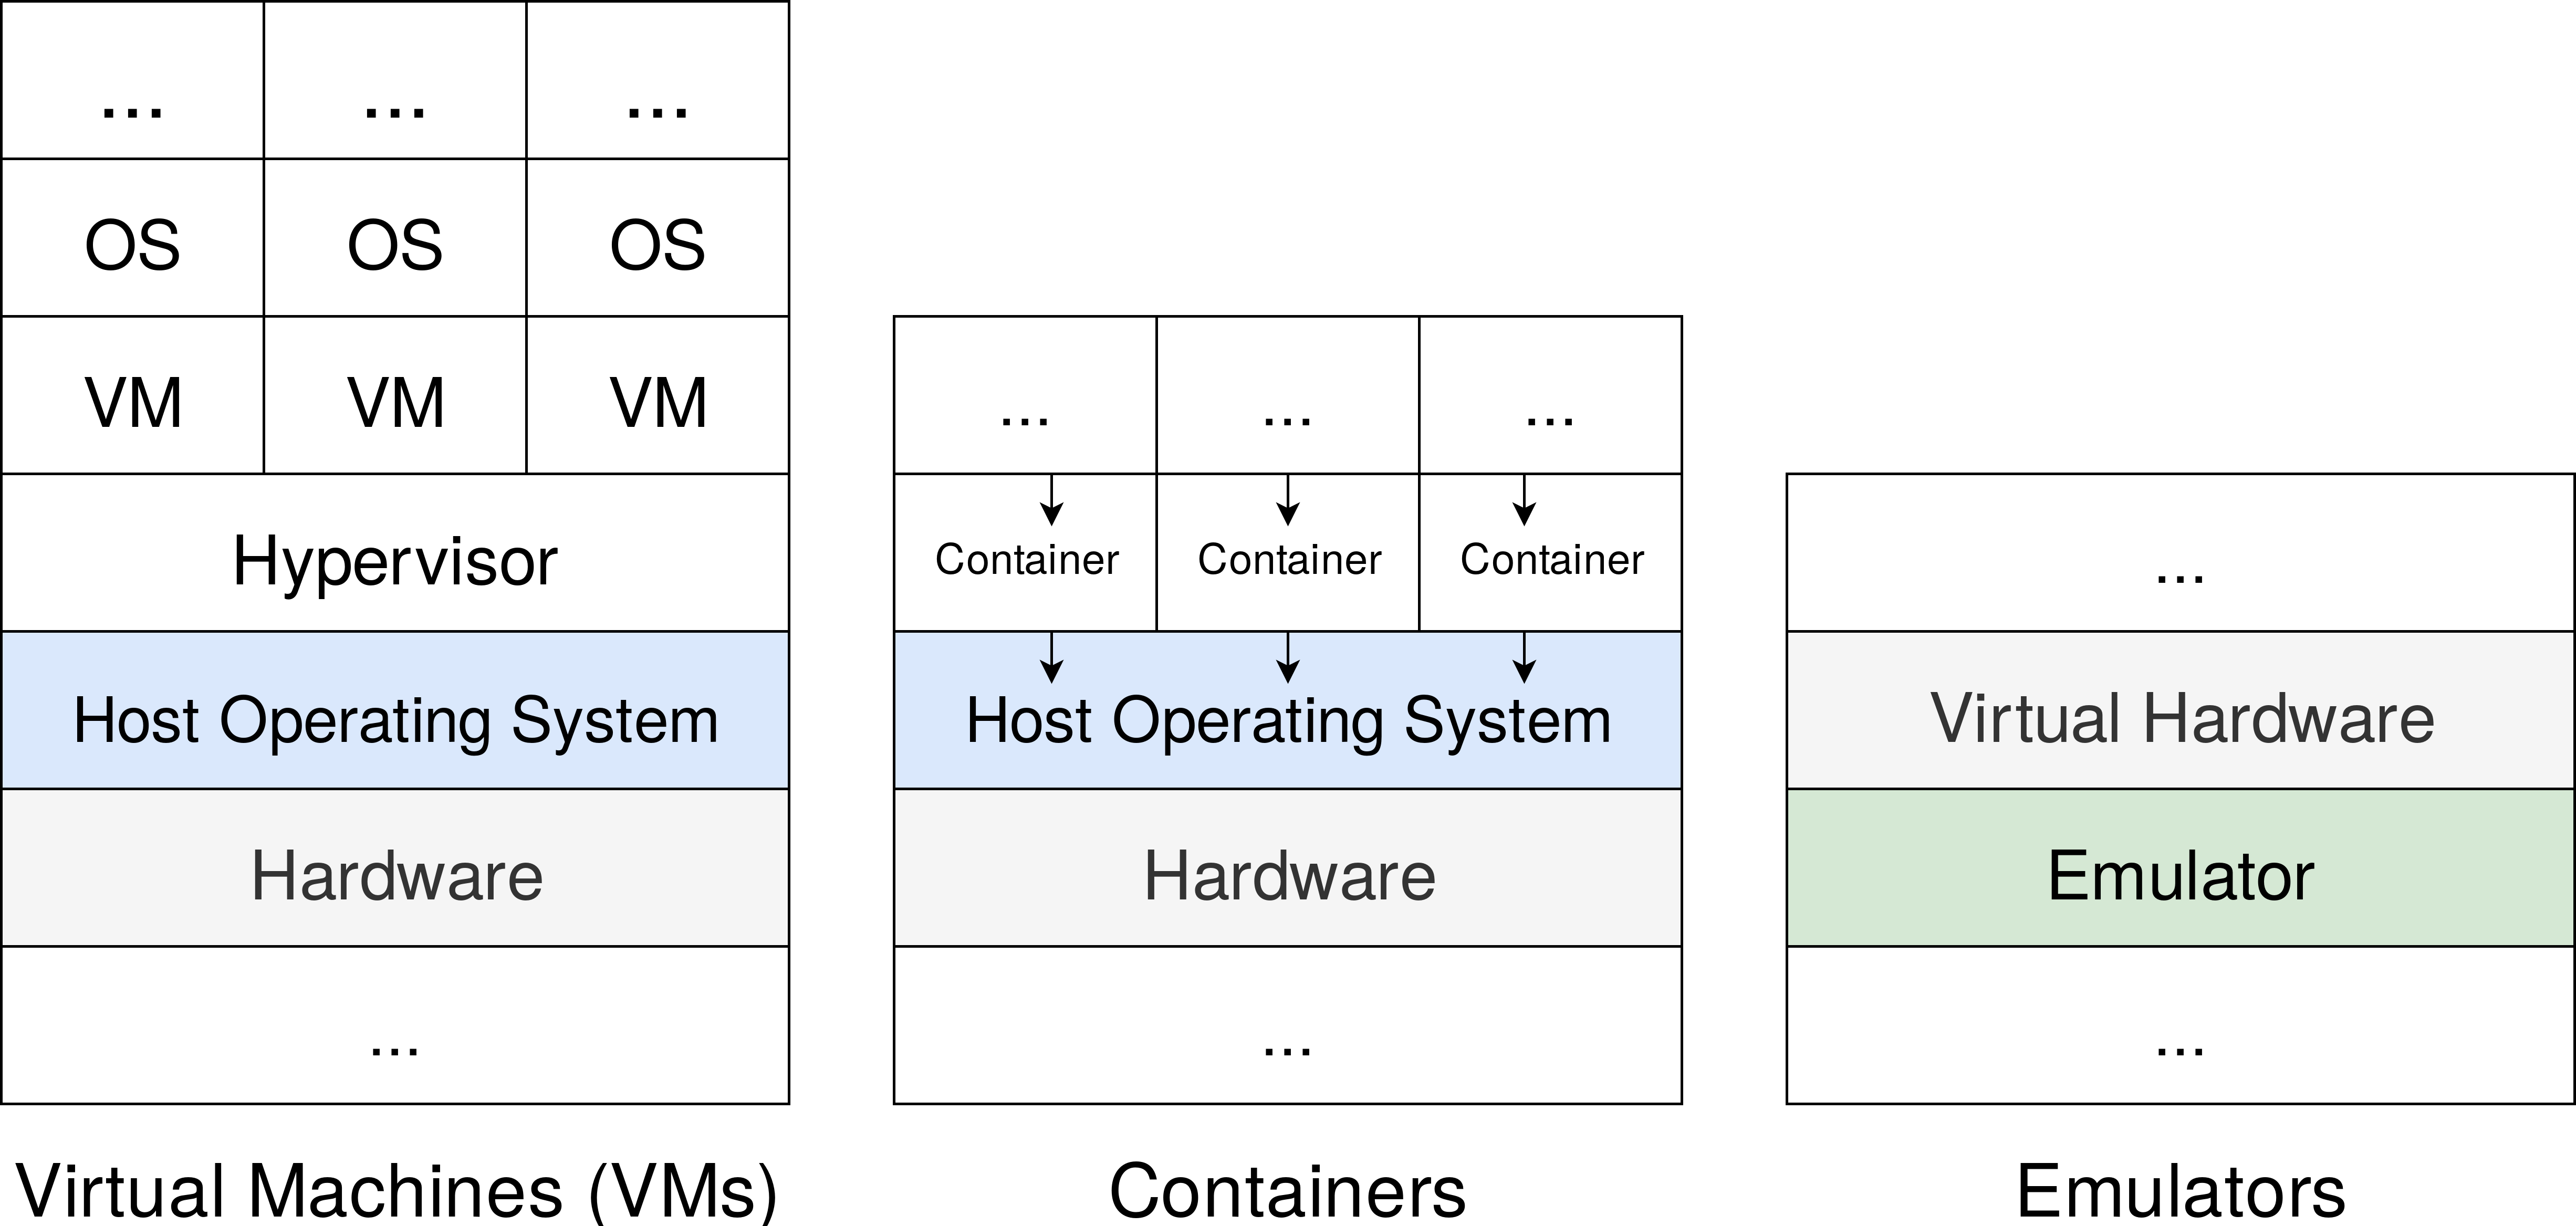
\includegraphics[width=0.70\textwidth]{vms_containers_emulators.png}
    \caption{Virtualization is a very resource expensive proposition. Containerization is cheaper, as it shares a kernel with the host OS. Emulation allows us to emulate hardware as software. Any of these methods can be used in conjunction with any other method.\vspace{-10}}
    \label{fig:vms_containers_emulators}
\end{figure}

\section{Containerization}\label{sec:containerization}

One of the challenges of distributed software development across heterogeneous platforms is the problem of variability. With the increasing pace of software development comes the added burden of software maintenance. As hardware and software stacks evolve, so too must source code be updated to build and run correctly. Maintaining a stable and well documented codebase can be a considerable challenge, especially in an academic setting where contributors are frequently joining and leaving the project. Together, these challenges present significant obstacles to experimental reproducibility and scientific collaboration.


\begin{figure}[ht]
    \centering
    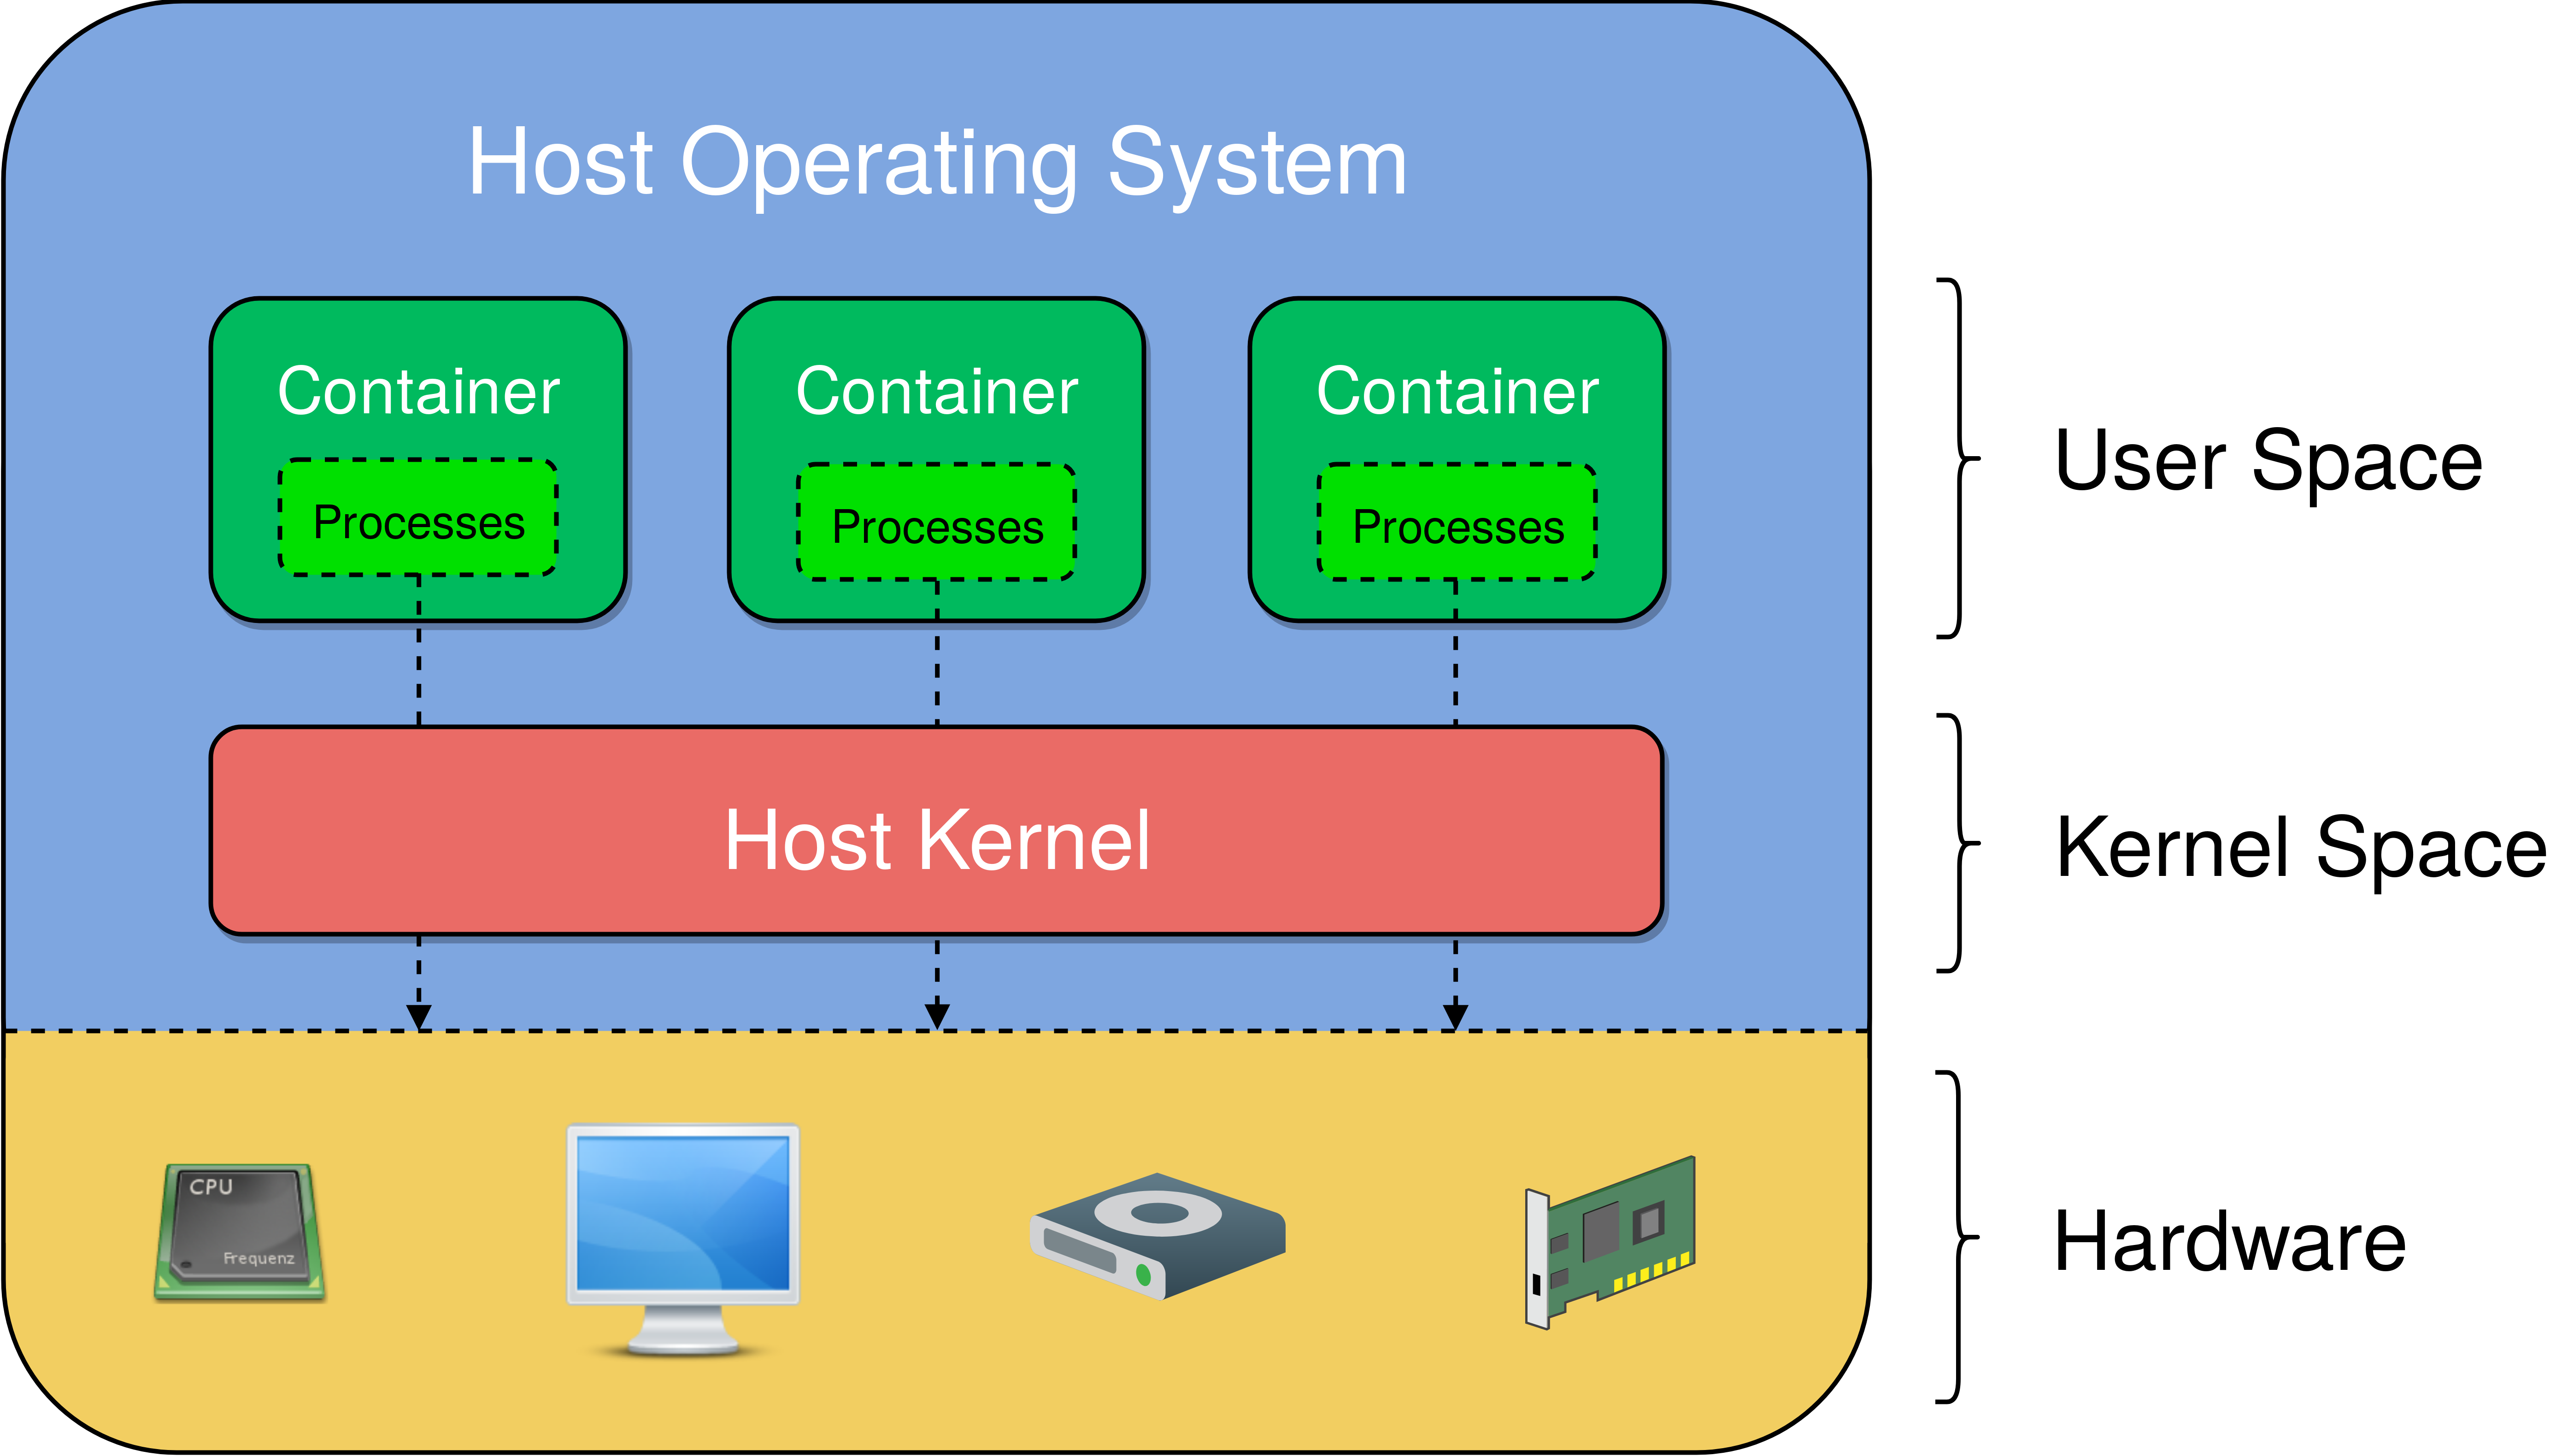
\includegraphics[width=0.65\textwidth]{user_kernel_hardware.png}
    \caption{Containers live in user space. By default they are sandboxed from the host OS and sibling containers, but unlike VMs, share a common kernel with each other and the host OS. All system calls are passed through host kernel.}
    \label{fig:user_kernel_hardware}
\end{figure}

Docker containers are sandboxed runtime environments that are portable, reproducible and version controlled. Each environment contains all the software dependencies necessary to run the packaged application(s), but remains isolated from the host OS and file system. Docker provides a mechanism to control the resources each container is permitted to access, and a separate Linux namespace for each container, isolating the network, users, and file system mounts. Unlike virtual machines, container-based virtualization like Docker only requires a lightweight kernel, and can support running many simultaneous containers with close to zero overhead. A single Raspberry Pi is capable of supporting hundreds of running containers.

While containerization simplifies the process of building and deploying applications considerably, it also introduces some additional complexity to the software development lifecycle. Docker, like most container platforms, uses a layered filesystem. This enables Docker to take an existing ``image'' and change it by installing new dependencies or modifying its functionality. Images may be based on a number of lower layers, which must periodically be updated. Care must be taken when designing the development pipeline to ensure that such updates do not silently break a subsequent layer as described earlier.

\begin{figure}[ht]
    \centering
    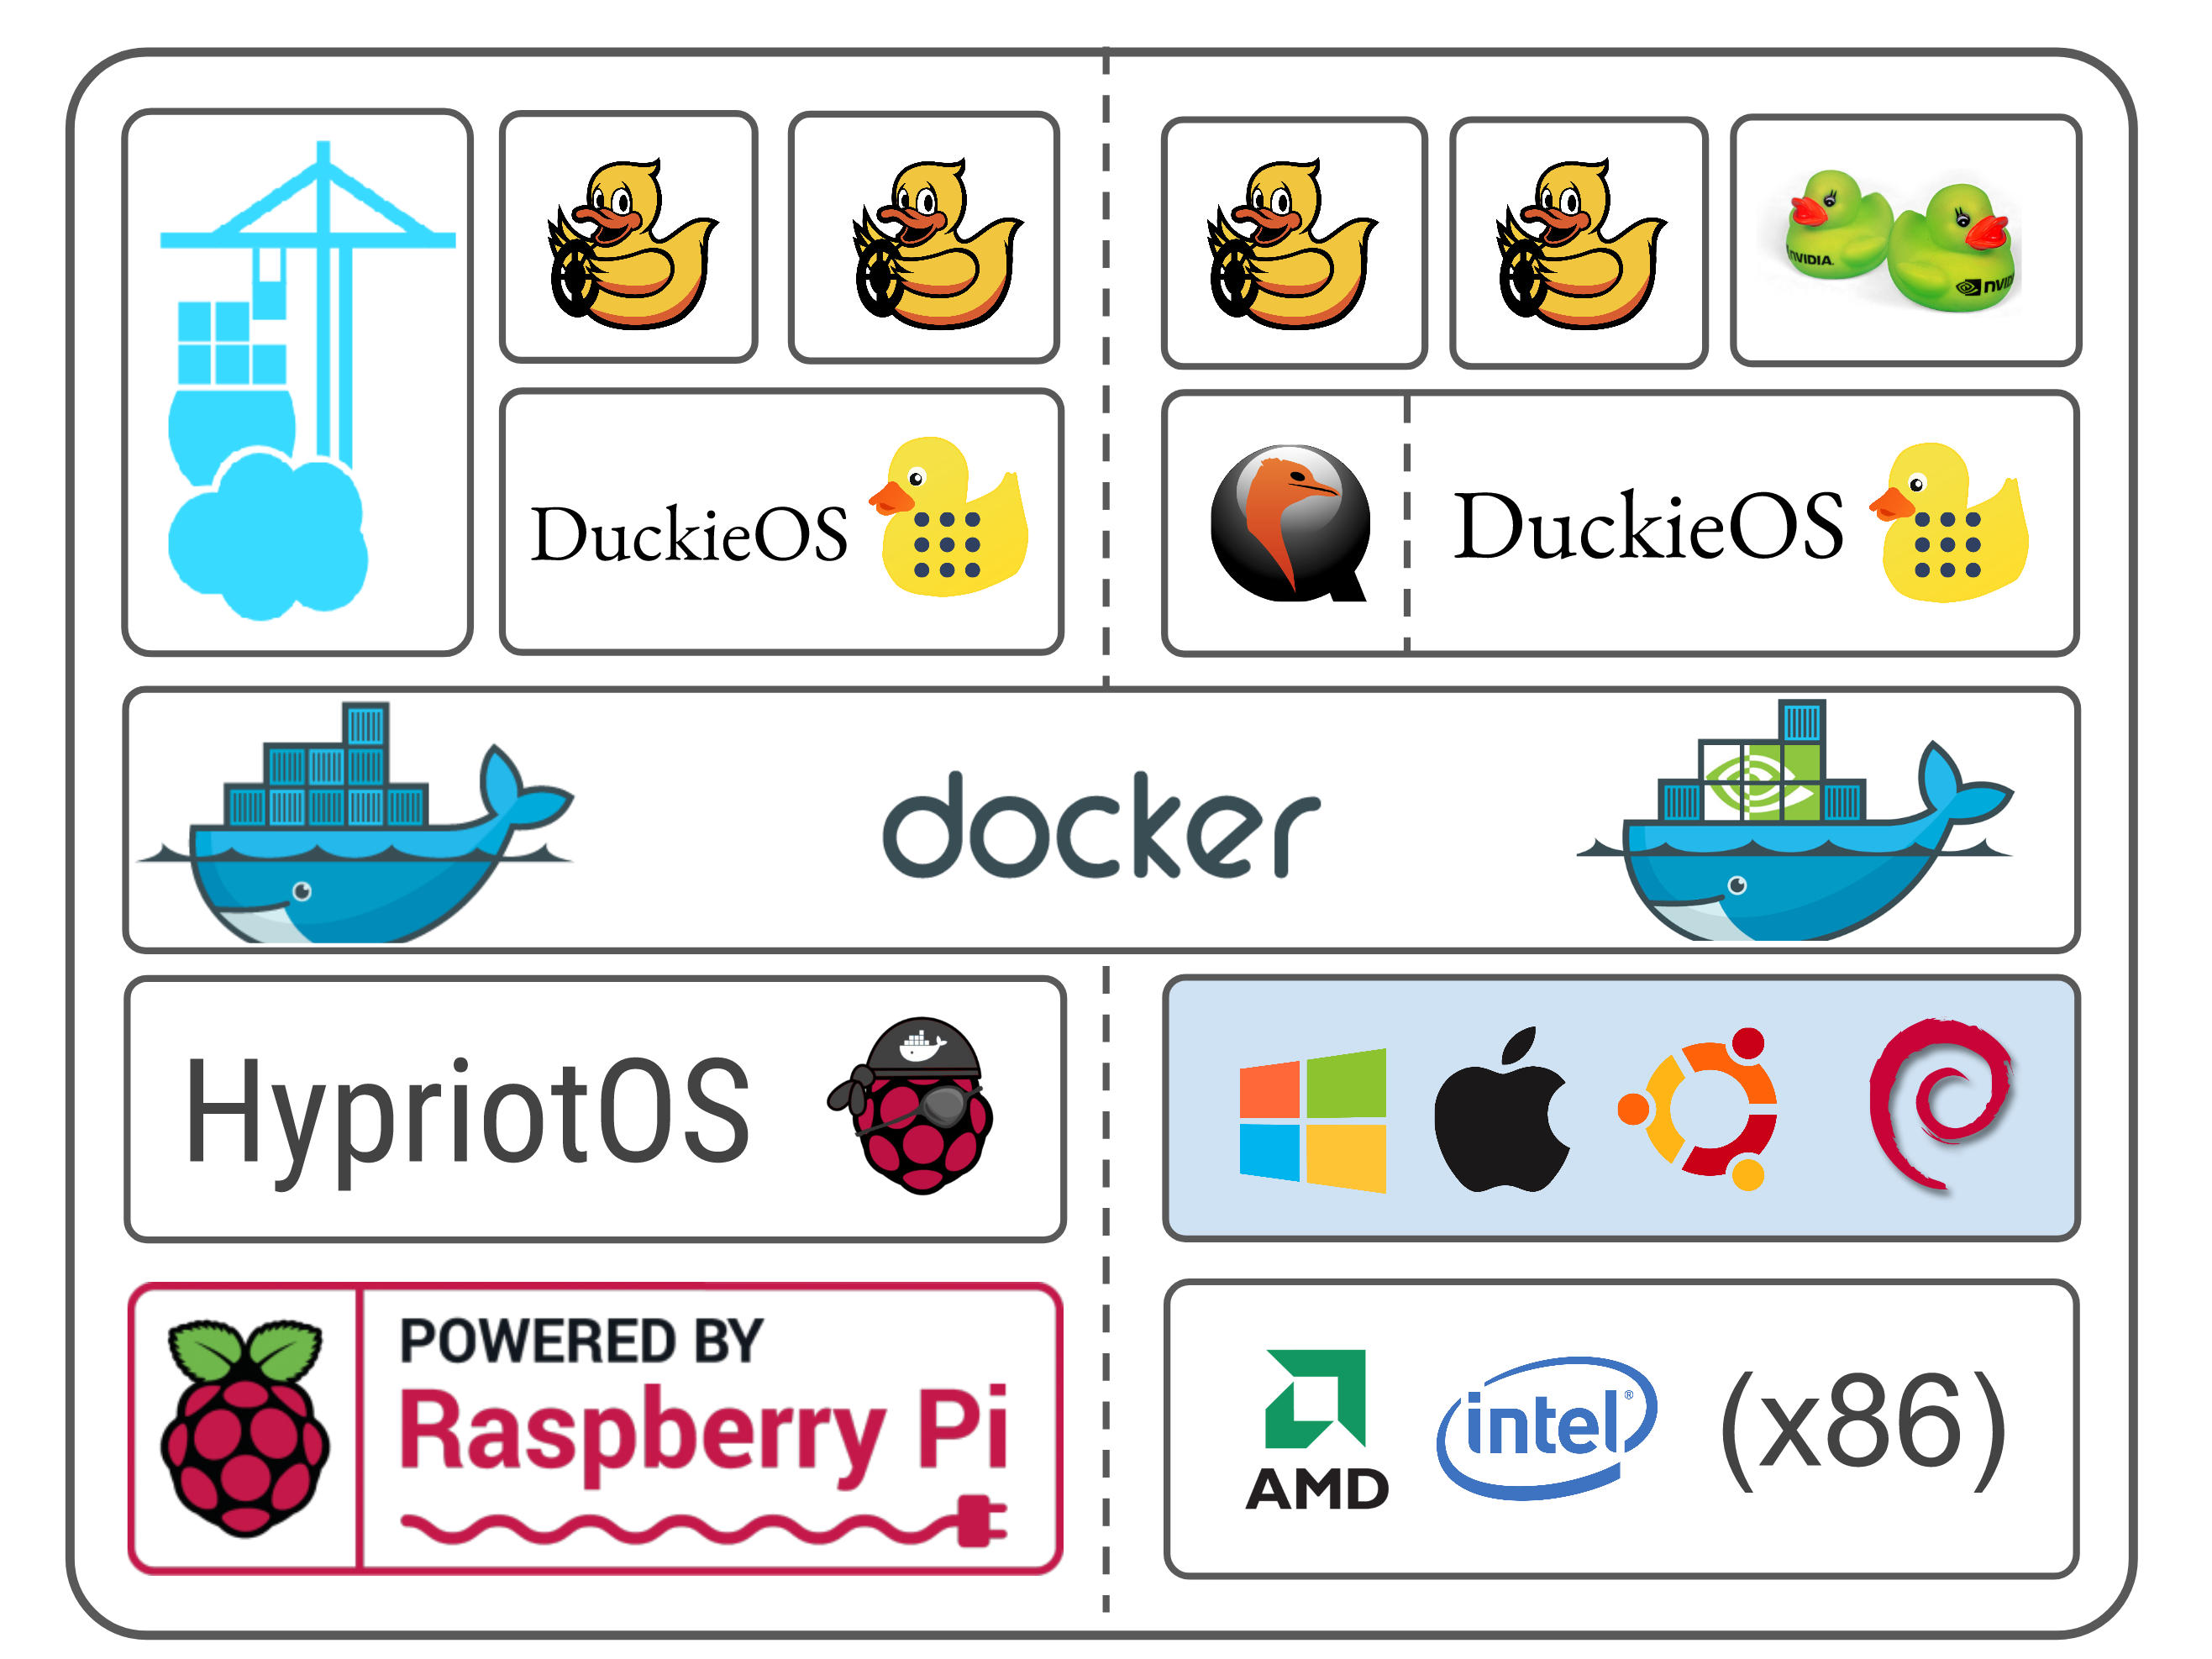
\includegraphics[width=0.50\textwidth]{docker_stack_1.png}
    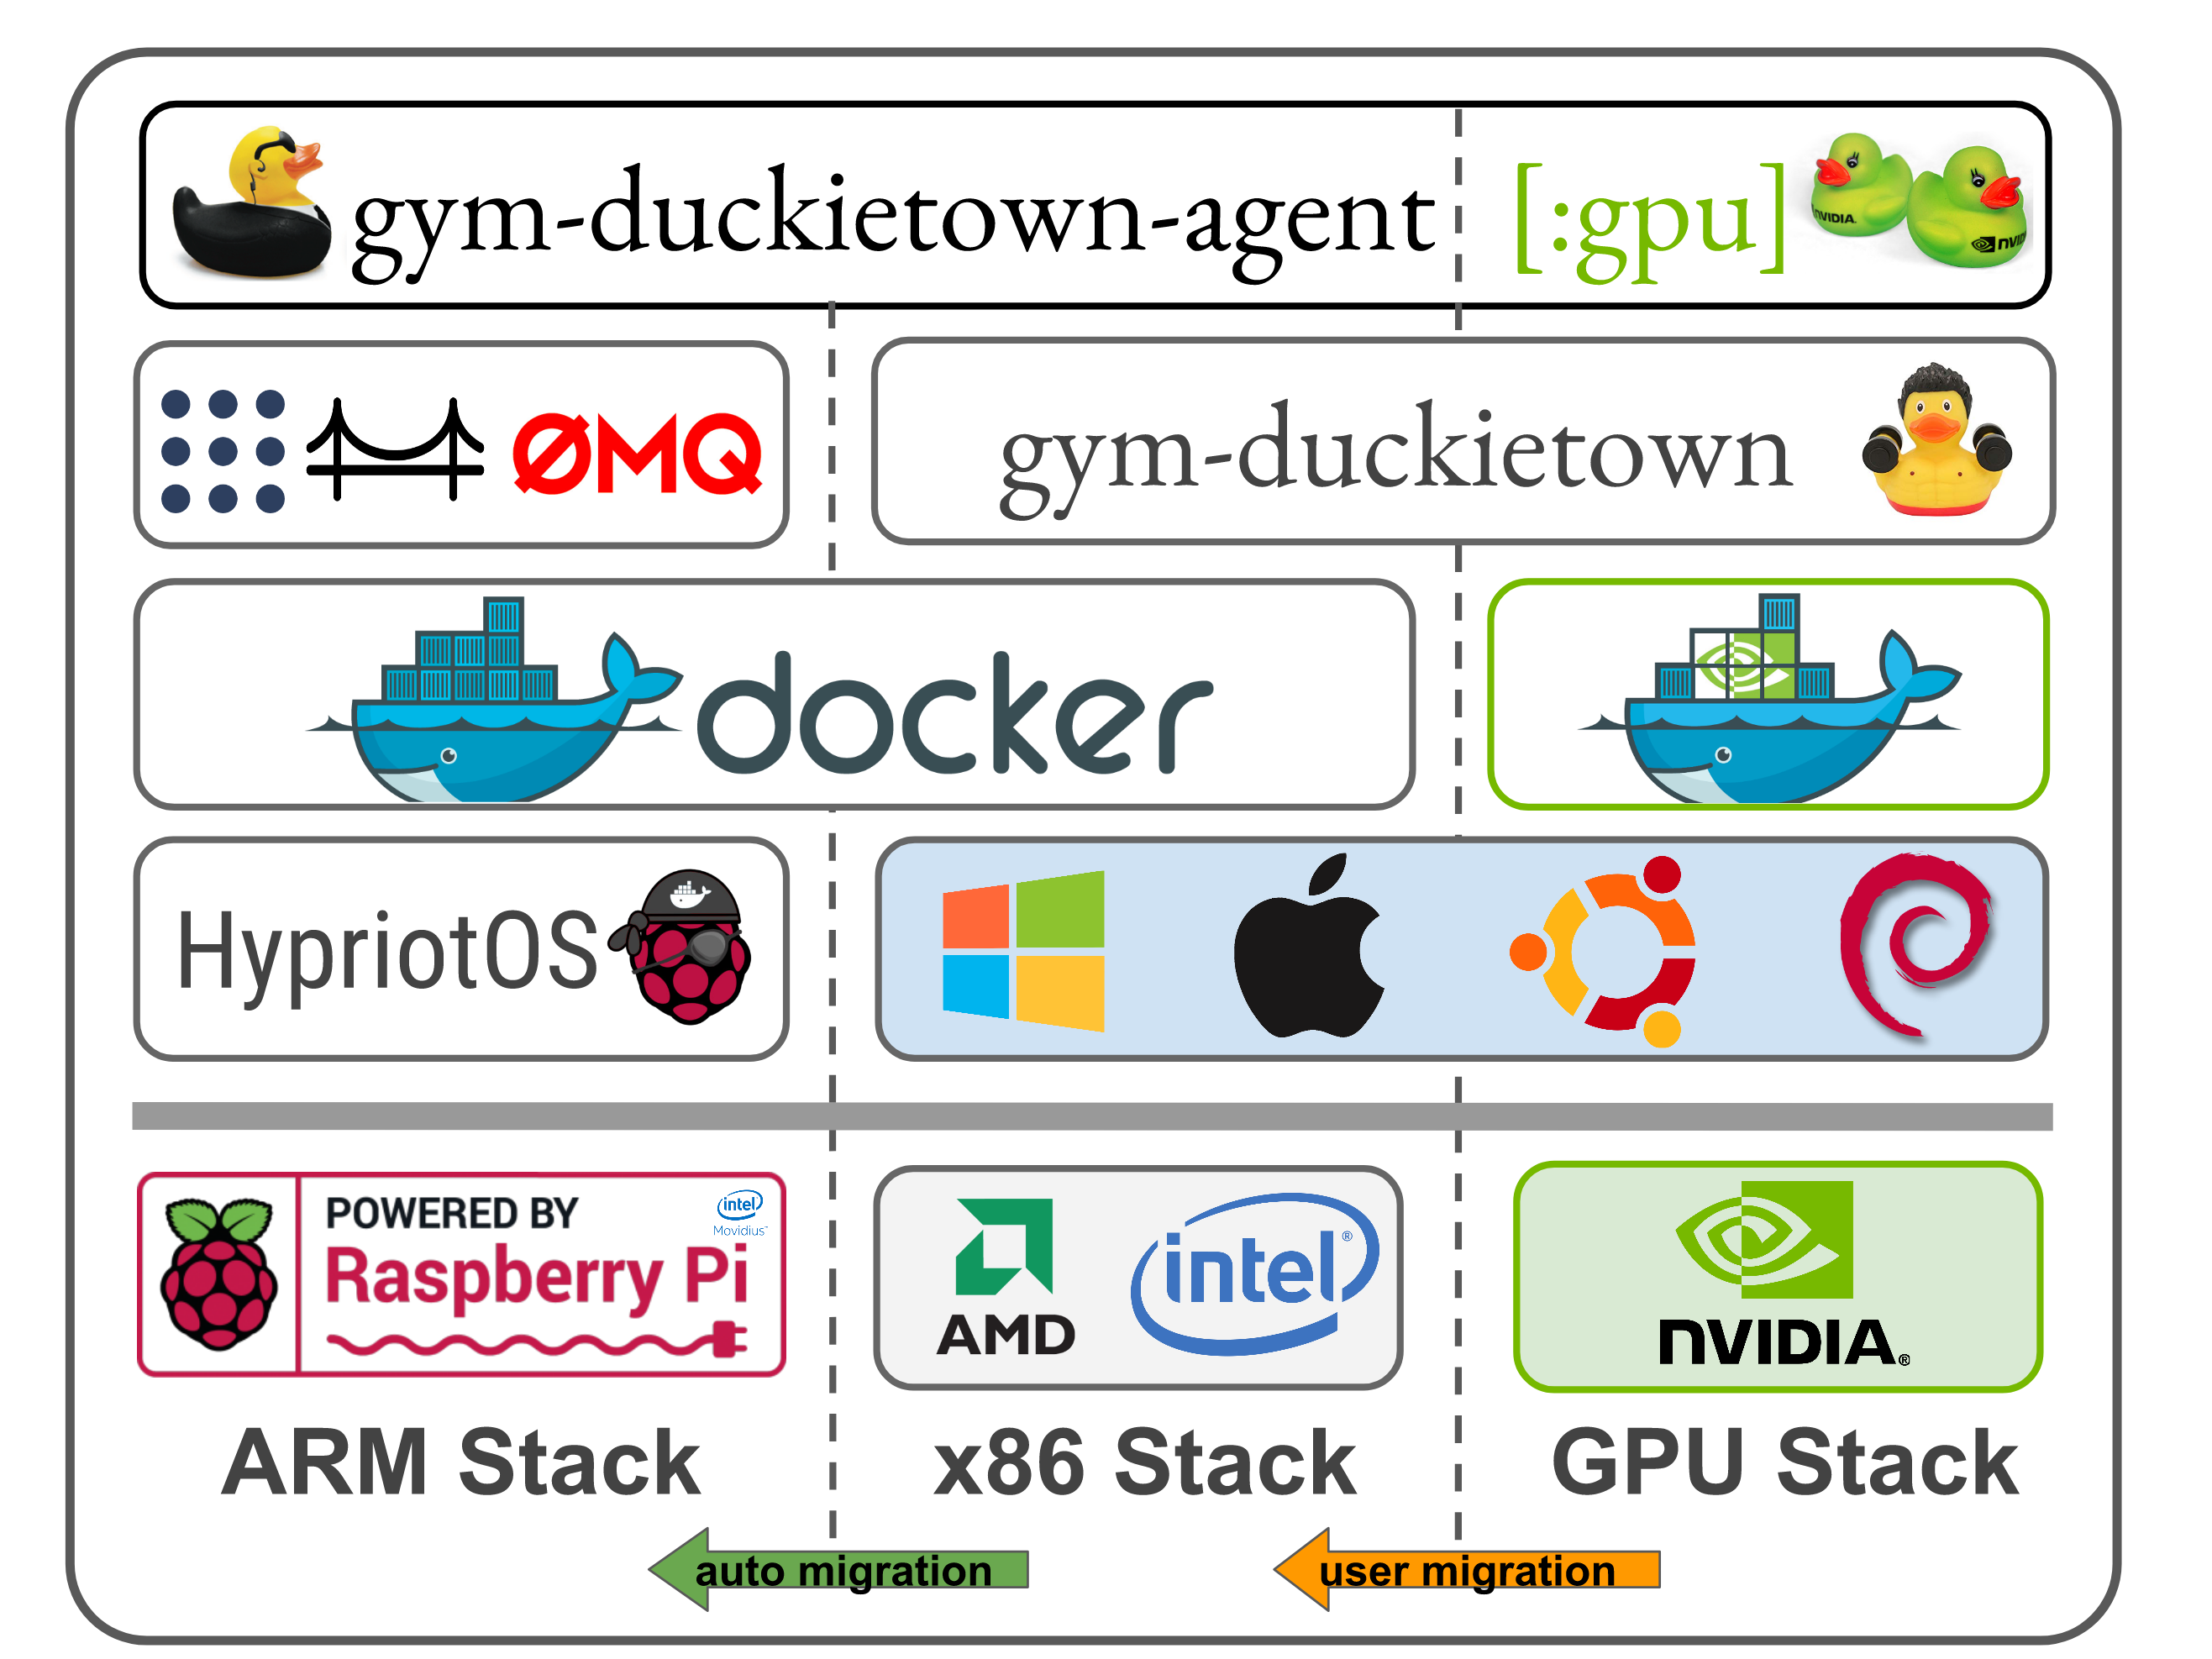
\includegraphics[width=0.50\textwidth]{docker_stack_2.png}
    \caption{AI-DO container infrastructure. Left: The ROS stack targets two primary architectures, x86 and ARM. To simplify the build process, we only build ARM artifacts, and emulate ARM on x86. Right: Reinforcement learning stack. Build artifacts are typically trained on a GPU, and transferred to CPU for evaluation. Deep learning models, depending on their specific architecture, may be run on an ARM device using an Intel NCS.}
    \label{fig:docker}
\end{figure}

\section{Docker and ROS}

Prior work has explored the Dockerization of ROS containers~\cite{white2017ros-docker}. This work forms the basis for our own, which is extended specifically for the Duckietown platform~\cite{paull2017duckietown}.

The Duckietown platform supports two primary instruction set architectures: x86 and ARM. To ensure the runtime compatibility of Duckietown packages, we cross-build using hardware virtualization to ensure build artifacts can be run on all target architectures. Runtime emulation of foreign artifacts is also possible, using a similar technique.\footnote{For more information, this technique is described in further depth at the following URL: \url{https://www.balena.io/blog/building-arm-containers-on-any-x86-machine-even-dockerhub/}.} For performance and simplicity, we only build ARM artifacts and use emulation where necessary (e.g., on x86 devices). On ARM-native, the base operating system is HypriotOS, a lightweight Debian distribution with built-in support for Docker. For both x86 and ARM-native, Docker is the underlying container platform upon which all user applications are run, inside a container.

\section{Conclusion}

One issue encountered is the matter of whether to package source code directly inside the container, or to store it separately. If source code is stored separately, a developer can use a shared volume on the host to build the artifacts. In this case, while build artifacts images may be standalone reproducible, they are not easily modified or inspected. The second method is to ship code directly inside the container, where any changes to the source code will trigger a subsequent rebuild, effectively tying the sources and the build artifacts together. Including source code alongside build artifacts has the benefit of improved reproducibility and diagnostics. If a competitor requires assistance, troubleshooting becomes much easier when the source code is directly accessible. However doing so adds some friction during development, which has caused competitors to struggle with environment setup. One solution is to store all sources on the local development environment and rebuild the Docker image periodically, copying sources into the image.

\rare{\chapter{Case study: application for autonomous robotics}\label{ch:case-study}}

As a case study, we have implemented a mobile application using ROS, Docker, and Android, using the proposed toolchain.

\section{Design}

Designed with Hatchery.

\section{Implementation}

Implementation includes Kotlin$\nabla$

\section{Verification and validation}

Verified using property-based testing.

\section{Containerization}

Deployed and CI-tested using Docker.

\rare{\chapter{Conclusion}\label{ch:conclusion}}

\section{Future work}

\subsection{Requirements Engineering}

Often it is not possible, or desirable to summarize the performance of a complex system using a single variable. In multi-objective optimization, we have the notion of pareto-efficiency...

Traditional software engineering has followed a rigorous process model and testing methodology. This model has guided the development of traditional software engineering, intelligent systems will require a re-imagining of these ideas to build systems that adapt to their environment during operation. Intelligent systems are designed with objective functions, which are typically one- or low-dimensional metrics for evaluating the performance of the system. Most often, these take the form of a single criteria, such as an \textit{error} or \textit{loss} which can represent descriptive phenomena such as latency, safety, energy efficiency or any number of objective measures.

For example, in the design of a web based advertisement recommendation system, we can optimize for various objectives such as click rate, engagement, sales conversion. So long as we can measure these parameters, with today's powerful function approximators, we can optimize for any single criterion or combination thereof. Much of the work involved in machine learning is to find representations which are amenable to learning, and preventing unintended consequences. For example, by optimizing for click rate, we create an artificial market for click bots. Similarly, in self driving cars, we often want to optimize for passenger safety. However by doing so naively, we create a vehicle that never moves, or always yields to nearby vehicles.

When building an intelligent system developers must first ask, "What are the requirements of the system?" This question is often the most troublesome part, because the requirements must not be fuzzy specifications like traditional software engineering, but precise, programmable directives. "The system must be fast," is not sufficiently precise. These kinds of requirements must be translated into statistical loss functions, so intelligent systems engineers must be very precise when specifying requirements. If we simply say, "The system must produce a valid response as quickly as possible, in less than 100ms," is better, but leaves open the possibility of returning an empty response.

In traditional software engineering, it is reasonable to assume the people who are implementing a system have some implicit knowledge and are generally well-intentioned human beings working towards the same goal. When building an intelligent system, a more reasonable assumption is that the entity implementing our requirements is a naive but powerful genie, and possibly an adversarial one. When given an optimization metric, it will take every available shortcut to meet that metric. If we are not careful about requirements engineering, this entity can produce a system that does not work, or has unintended consequences.

In the strictest sense, designing a good set of requirements is indistinguishable from implementing the system. With the right language abstractions (e.g.\ declarative programming), requirements and implementation can be the same thing. These ideas have been explored in recent decades with languages like SQL and Prolog. While these are toy systems, neural networks can express much larger classes of functions than traditional software engineering.

\subsection{Continuous Delivery and Continual Learning}

An overall trend in software and systems engineering is the transition away from long development cycles towards continuous integration and deployment. Development teams in the industry are encouraged to iterate in a series of short sprints between feature development and deployment. In some cases, software is shipped to users on a nightly basis, with automated testing and deployment. Similarly, intelligent systems have a need to continuously adapt to their environment, and will change their code on an even shorter basis.

Incremental updates will grow increasingly smaller, until the program starts to alter itself after every input it processes.

We need tools to more effectively harness the stochasticity of these learning systems.

\subsection{Developers, Operations, and the DevOps toolchain}

Software engineers have begun to realize the value of bespoke tools that facilitate the process of shipping software, in addition to the software itself.

Teams building software are cybernetic systems, and require meta-programs for building code and organizational processes which enable them to ship code more efficiently.

\bibliography{thesis}
\bibliographystyle{plain}
\end{document}